\documentclass[FM,BP,fonts]{tulthesis}

\newcommand{\verze}{2.0}

\usepackage{polyglossia}
\setdefaultlanguage{czech}
\usepackage{xevlna}

\usepackage{makeidx}
\makeindex
\usepackage{hyperref}

\usepackage{xunicode}
\usepackage{xltxtra}
\usepackage{mathtools}
\usepackage{graphicx}
% příkazy specifické pro tento dokument
\newcommand{\argument}[1]{{\ttfamily\color{\tulcolor}#1}}
\newcommand{\argumentindex}[1]{\argument{#1}\index{#1}}
\newcommand{\prostredi}[1]{\argumentindex{#1}}
\newcommand{\prikazneindex}[1]{\argument{\textbackslash #1}}
\newcommand{\prikaz}[1]{\prikazneindex{#1}\index{#1@\textbackslash #1}}
\newenvironment{myquote}{\begin{list}{}{\setlength\leftmargin\parindent}\item[]}{\end{list}}
\newenvironment{listing}{\begin{myquote}\color{\tulcolor}}{\end{myquote}}
\sloppy

% deklarace pro titulní stránku
\TULtitle{Predikce profilů spotřeby elektrické energie}{Prediction of power consumption profiles}
\TULauthor{Pavel Vácha}

% pro bakalářské, diplomové a disertační práce
\TULprogramme{B0613A140005}{Informační technologie}{Information Technology}
\TULbranch{B0613A140005AI-80}{Aplikovaná informatika}{Applied informatics}
\TULsupervisor{Ing. Jan Kraus, Ph.D.}

\TULyear{2024}

\usepackage[backend=biber,urldate=short,style=iso-numeric]{biblatex}
\bibliography{refs}
\usepackage[none]{hyphenat}

%\usepackage[ 
%backend=biber
%% ,style=iso-authoryear % styl vyžaduje FZS TUL , místo příkazu \cite{} je potřeba využít \parencite{} (sazba kulatých závorek) / style required by FZS TUL use \parencite{} instead of \cite{}
%,style=iso-numeric
%%,style=numeric
%%,sortlocale=cs_CZ
%,autolang=other
%,bibencoding=UTF8
%%,urldate=edtf
%,maxcitenames=2 %maximum v textu citovaných jmen
%,maxbibnames=3 %maximum v seznamu vyjmenovaných autorů
%]{biblatex}
%\addbibresource{refs.bib}% vložení seznamu literárních zdrojů v bib formátu / input of references in bib format
%% Úprava iso-numeric.bbx v souladu s požadavky TUL hranaté závorky v číslovaném seznamu / Modification of iso-numeric.bbx in accordance with TUL requirements of square brackets in a numbered list
%\DeclareFieldFormat{labelnumberwidth}{\mkbibbrackets{#1}}



%\DeclareDelimFormat{finalnamedelim}{%
%	\ifnumgreater{\value{liststop}}{2}{\finalandcomma}{}%
%	\addspace\bibstring{and}\space}





\usepackage{listings}
\usepackage{caption}
\usepackage{color}

\definecolor{dkgreen}{rgb}{0,0.6,0}
\definecolor{gray}{rgb}{0.5,0.5,0.5}
\definecolor{mauve}{rgb}{0.58,0,0.82}

\renewcommand{\lstlistingname}{Zdrojový kód}

\lstset{frame=tb,
	language=Python,
	aboveskip=3mm,
	belowskip=3mm,
	showstringspaces=false,
	columns=flexible,
	basicstyle={\small\ttfamily},
	numbers=none,
	numberstyle=\tiny\color{gray},
	keywordstyle=\color{blue},
	commentstyle=\color{dkgreen},
	stringstyle=\color{mauve},
	breaklines=true,
	breakatwhitespace=true,
	tabsize=3,
	captionpos=b
	%,
	% caption={My Code Listing},
}




\begin{document}

\ThesisStart{male}
%\ThesisStart{zadani-a-prohlaseni.pdf}

\begin{abstractCZ}
Tato práce se zabývá problematikou krátkodobých a střednědobých predikcí spotřeby elektrické energie pomocí hlubokých neuronových sítí a dalších metod strojového učení.  
Finální modely jsou natrénovány na datových sadách poskytnuté společností Albistech a na veřejných datech společnosti UK Power Networks. Datové sady byly očištěny a byla na nich provedena explorační analýza pro dosažení lepších výsledků.
Výsledky ukazují, že finální modely dokáží předpovídat až s 95\% přesností v rámci jednoho dne a dokáží tak poskytnout spolehlivé výsledky pro budoucí implementaci v informačním systému NEO a poskytnout tak zákazníkům nástroj pro efektivnější hospodaření.
\end{abstractCZ}

\begin{keywordsCZ}
spotřeba energie, analýza časových řad, predikce, parametrické modelování, strojové účení

\end{keywordsCZ}

\vspace{2cm}

\begin{abstractEN}
This thesis explores the issue of short and medium term forecasting of electricity consumption using deep neural networks and other machine learning methods.
The final models are trained on datasets provided by Albistech and UK Power Networks public data. The datasets were cleaned and exploratory data analysis was performed to obtain better results.
The results show that the final models can forecast with up to 95\% accuracy within one day, and can thus provide reliable results for the future implementation in the NEO system and provide customers with a tool for more efficient management.
\end{abstractEN}

\begin{keywordsEN}
energy consumption, time series analysis, forecasting, parametric modeling, machine learning
\end{keywordsEN}

\clearpage

\begin{acknowledgement}
Rád bych poděkoval všem, kteří přispěli ke vzniku tohoto díla. Zejména společnosti Albistech s.r.o za poskytnutá data a zázemí pro vypracování práce.
\end{acknowledgement}

\tableofcontents

\clearpage

\listoffigures

\listoftables

\clearpage


\begin{abbrList}
\textbf{LSTM} & Long-short term memory, architektura rekurentní neuronové sítě \\
\textbf{CNN} & Convolutional Neural Network, konvoluční neuronová síť \\
\textbf{MSE} & Mean squared error, střední kvadratický chyba \\
\textbf{MAE} & Mean average error, průměrná absolutní odchylka \\
\textbf{MAPE} & Mean average error, průměrná procentuální absolutní odchylka \\
\textbf{RMSE} & Root mean squared error, směrodatný odchylka \\
\textbf{ReLU} & Rectifed Linear Unit, aktivační funkce \\
\textbf{GBT} & Gradient boosted trees, gradientní boostované stromy \\
\textbf{EDA} & Exploratory data analysis, explorační datová analýza

\end{abbrList}

\chapter{Úvod}


Vzorce spotřeby a jejich dopady na naše životní prostředí jsou aktuálně mezi největ-
šími výzvami naší doby. Díky pochopení jak a kdy lidé spotřebovávají energii a jak

se tyto vzorce mění, jsme schopni zajistit udržitelnou budoucnost.
Tradiční modely spotřeby se obvykle opírají o národní nebo globální data, která

nemusí zcela odrážet lokální vzorce spotřeby nebo jejich podmínky (např. klimatic-
ké). Naproti tomu modely lokální spotřeby mohou poskytnout přesnější a mnohem

relevantnější informace pro konkrétní region či oblast.
V tomto projektu si kladu za cíl vyvinout model lokální spotřeby založený na
historických datech spolu s environmentálními parametry, pokud jsou pro danou
oblast dostupné. Tento model může být velmi cenný pro plánování a implementaci
udržitelných opatření v oblasti energetiky a ochrany životního prostředí. Získání
přesnějšího a místně relevantního pohledu na spotřebu energie nám umožní přijímat
informovaná rozhodnutí a přizpůsobit naše strategie tak, aby byly co nejefektivnější
a nejohleduplnější k životnímu prostředí.
Pro vytvoření spolehlivého a vhodného modelu lokální spotřeby se část tohoto
projektu bude zabývat rešerší různých technik strojového učení spolu s metodami
ze statistické analýzy.


\chapter{Časové řady}
Spotřeba energie v domácnostech může být chápána jako posloupnost měření, kde každý jednotlivý záznam je v určitém časovému okamžiku. Před samotným průzkumem prediktivních metod je nutné si definovat několik pojmů z oblasti analýzy časových řád, které se budou v následujících kapitolách vyskytovat.

Časová řada je definována jako množina pozorování $x_t$, kde každé pozorování má záznam v čase $t$. \ref{neoc}. Příkladem typické časové řady může být vývoj ceny akcií na burze v čase nebo výše zmíněna spotřeba energie. Každá časová řada se dá rozložit (dekomponovat) na několik jednotlivých složek (komponent). 


\section{Komponenty časové řady}
Dekompozice časové řady umožňuje získat jednotlivé komponenty, jenž odhalují určité vlastnosti časové řady. Tyto komponenty a informace co nesou, jsou poté užitečné při samotné analýze a následné predikci časové řady.

\subsection{Trendová komponenta}
Tato komponenta zachycuje celkový dlouhodobý směr zkoumaného jevu časové řady. Trend může být rostoucí, klesající a nebo kompletně bez trendu. V kontextu této práce může být tato složka ovlivněna různými faktory, jako jsou změny v ekonomice, demografii nebo technologický pokrok. Označuje se jako $T_t$.

\subsection{Sezónní komponenta}
Sezónní komponenta $S_t$ určuje krátkodobý vzor, který se opakuje v pravidelných intervalech, avšak s frekvencí rok a méně. \ref{aha} V kontextu spotřeby energie v domácnostech může tato složka zahrnovat sezónní vzory spojené s ročními změnami, jako je zvýšená spotřeba v zimním období kvůli vytápění nebo v letním období kvůli klimatizaci. Tato složka bude klíčová pro identifikaci střednědobých cyklů spotřeby energie.

\subsection{Cyklická komponenta}
Analýza této cyklické komponenty $C_t$ může být klíčová při zkoumání vlivu širších socioekonomických faktorů na dlouhodobou spotřebu energie v domácnostech. Tato složka totiž představuje dlouhodobější vzory, jejichž frekvence přesahuje minimálně jeden rok. \ref{a} Zpravidla vyjadřuje kolísání okolo trendové komponenty.


\subsection{Náhodná komponenta}
 Jedná se o náhodné výkyvy, které nemohou být předpovězeny pomocí předchozích komponent a mohou být způsobeny různými nepředvídatelnými událostmi, jako jsou chyby v měření nebo neočekávané výpadky dodavatele energie. Zpravidla se značí jako  $\epsilon_t$.
 

\section {Stacionariata}
Pro analýzu časové řady je vhodné (pro většinu analýz podmínkou), aby řada byla takzvaně stacionární. Za stacionární časové řady se považují takové řady, které nemají trend, mají s měnícím se časem stejný rozptyl a stejný průběh autokorelační funkce. Tyto vlastnosti usnadňují predikci budoucích hodnot a proto je snaha převést řadu na stacionární. 

Nejjednodušší transformace řady na stacionární je pomocí diferencování. Tato transformace přispívá ke snížení trendové složky. Například diferenci prvního řádu se zapisuje jako:  
\begin{equation}
 \Delta x_t = x_t - x_{t-1}
\end{equation}
kde $x_t$ je hodnota v čase $t$ a $x_{t-1}$ je vzorek předcházející. Při analýze následující řady níže, kde je vidět lineární rostoucí trend, je třeba provést diferenci, aby tento trend zmizel.
 
\begin{figure}[htbp]
	\centering
	\makebox[\textwidth][c]{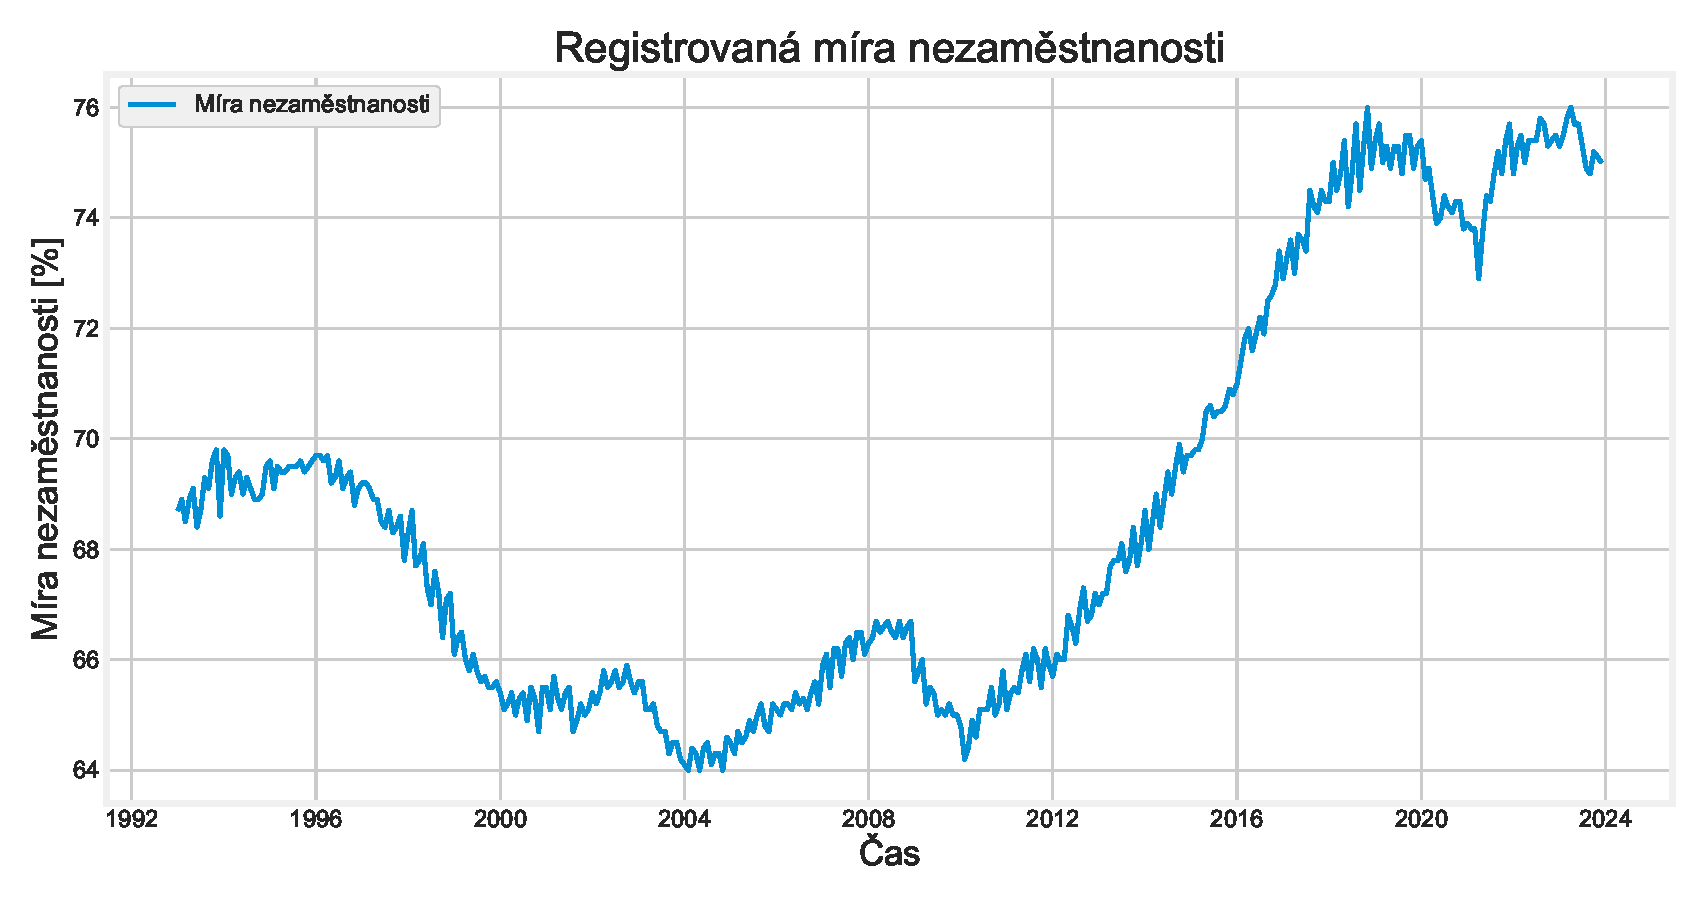
\includegraphics[width=0.7\textwidth]{pv_eg_02_mira_nezam.eps}}%
	\caption{Míra registrované nezaměstnanosti v ČR od roku 1993 }
	\label{fig:nezamestnanost}
\end{figure}

Po aplikaci diference prvního řádu lze vidět, že řada již nemá zjevný rostoucí trend a bylo by možné pokračovat v další analýze.

\begin{figure}[htbp]
	\centering
	\makebox[\textwidth][c]{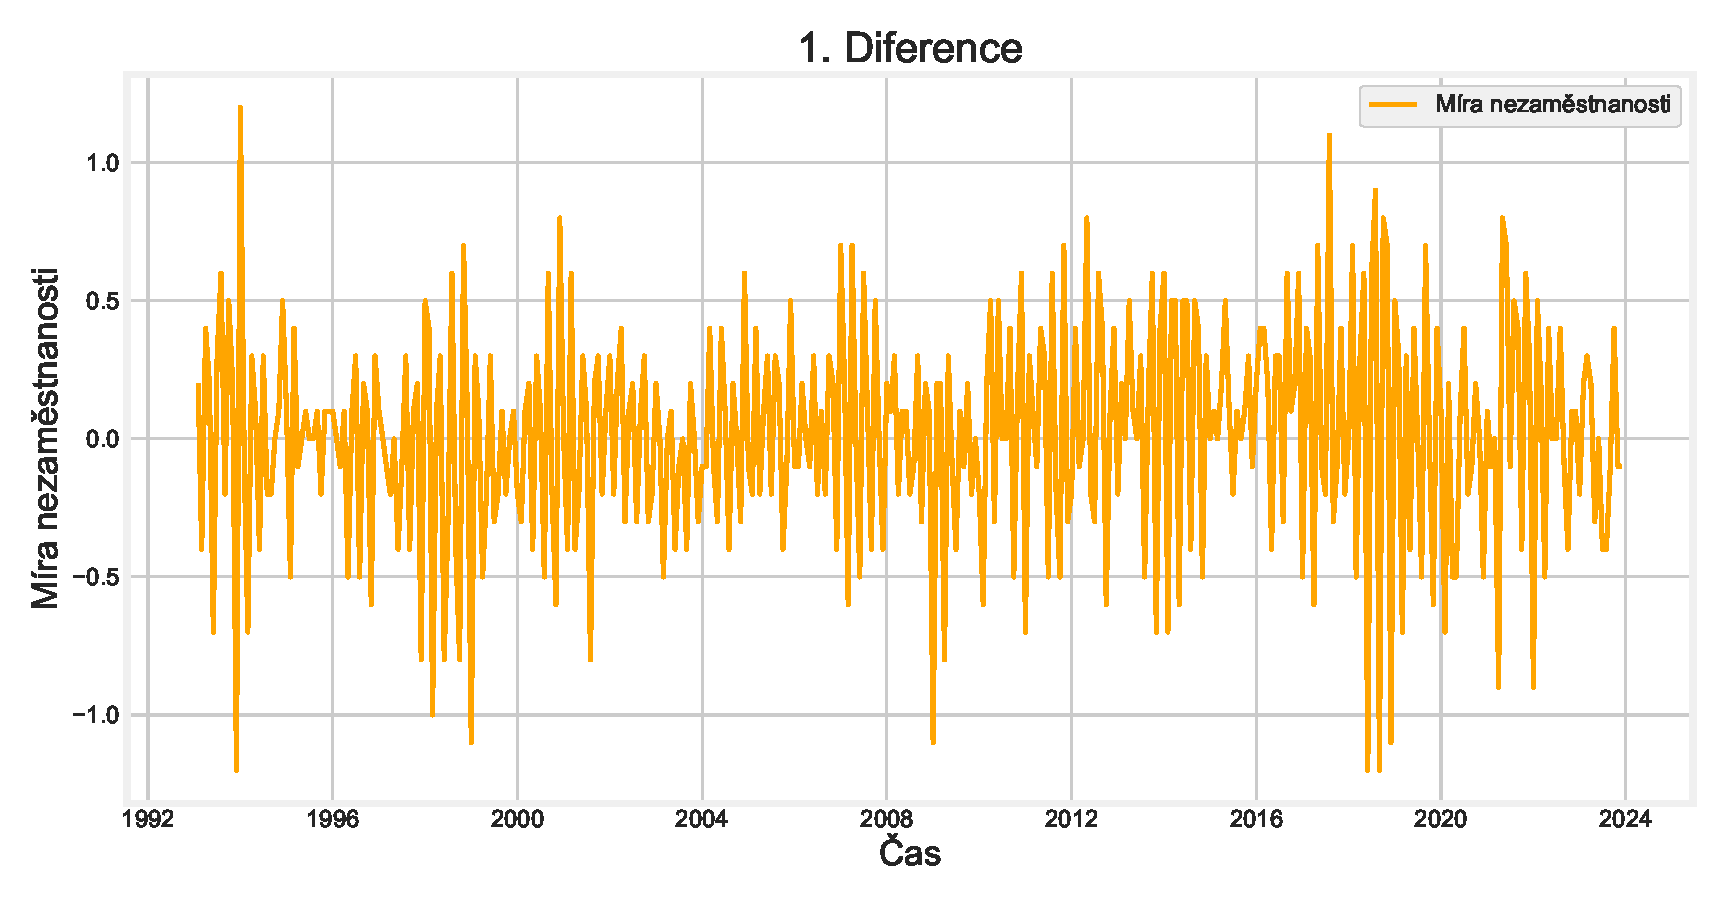
\includegraphics[width=0.7\textwidth]{pv_eg_02_mira_nezam_diff.eps}}%
	\caption{Míra registrované nezaměstnanosti po spočtení první diference }
	\label{fig:nezamestnanost_diff}
\end{figure}

Pro otestování zdali je řada stacionární existuje několik testů ze statistické analýzy. V implementační části této práci bude využito Dickey-Fullerova testu pro ověření stacionarity dat, nad kterými bude autor práce tvořit jednotlivé modely. 


\section{Dekompozice časové řady}
Jak bylo zmíněno výše, dekompozice umožňuje rozložit časovou řadu na jednotlivé komponenty. Z těch poté lze lépe pochopit, jakým způsobem se v časové řadě projevuje trend a sezónní variabilita. To je užitečné pro interpretaci dat a odhalení skrytých trendů nebo sezónních vzorů, což může být klíčové pro predikci a optimalizaci energetické efektivity v domácnosti.

Někdy se samotné komponenty po dekompozice využívají k predikci, obzvlášť pokud je trend jednoduchý. Lze ho totiž lépe predikovat, a stejně tak i sezónní vzory. \ref{}

Pro dekompozici se zpravidla používají dva základní modely, a to aditivní a multiplikativní. Volba modelu závisí na charakteru sezónnosti a trendu v časové řadě.

\subsection{Aditivní model}
Pro tento model se předpokládá, že řadu lze rozložit jako součet jednotlivých komponent.

\begin{equation}
	x_t = T_t + S_t + C_t + \epsilon_t
\end{equation}
kde $x_t$ je samotná hodnota časová řady v čase $t$.


\subsection{Multiplikativní model}
Analogicky tento model naopak předpokládá, že řadu lze rozložit jako součin jednotlivých komponent.
\begin{equation}
	x_t = T_t * S_t * C_t * \epsilon_t
\end{equation}

Tento model se využívá, pokud se výkyvy sezonní složky vůči trendu mění v čase.

 
\subsection{Klouzavý průměr}
Tento jednoduchý výpočet, který je schopen zvýraznit trend-cyklickou složkou, je jednou z nejjednodušších metod dekompozice. Mimo jiné dokáže vyhladit časovou řadu od krátkodobých výkyvů. Spočívá v jednoduchém průměrování různých pozorování a nebo celé řady.  Klouzavý průměr řádu $m$ lze zapsat jako:
 
\begin{equation}
SMA_m = \frac{1}{m} \sum_{i=-k}^{k}x_{t+i}
\end{equation}
 
kde $k$ se používá k určení, kolik hodnot před a po aktuálním čase $t$ se zahrne do výpočtu klouzavého průměru. Platí, že $m = 2k+1$

\begin{figure}[htbp]
	\centering
	\makebox[\textwidth][c]{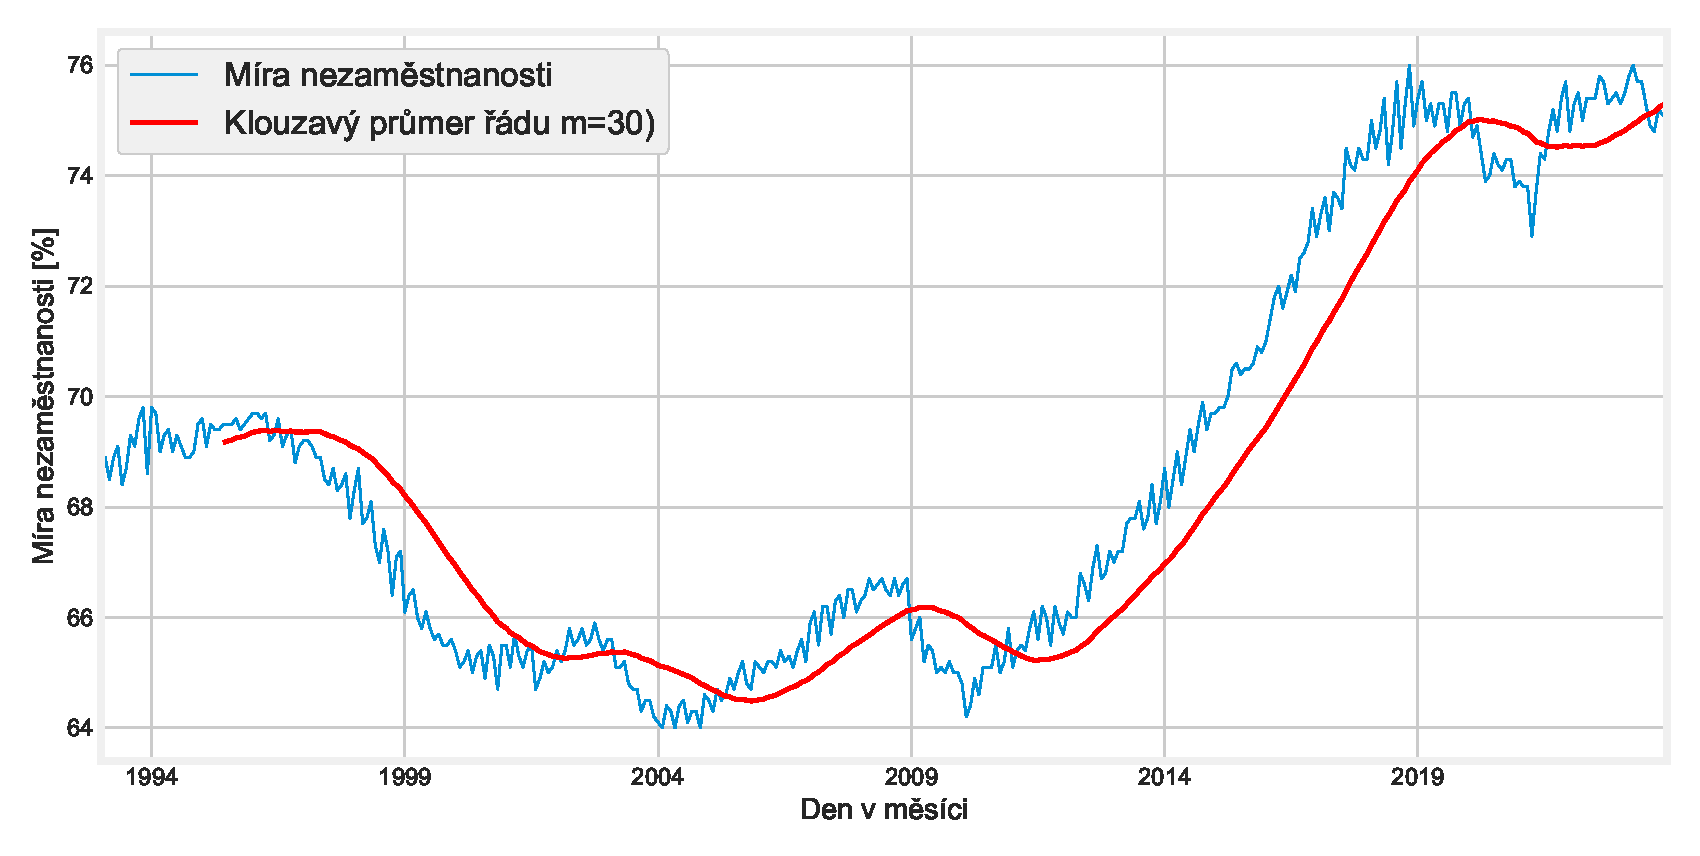
\includegraphics[width=1.0\textwidth]{pv_eg_01_moving_average.eps}}%
	\caption{Klouzavý průměr řádu m=30 popisující míru nezaměstnanosti v ČR od roku 1993. }
	\label{fig:my_graph}
\end{figure}

Na grafu výše lze vidět, že klouzavý průměr (červená čára) s řádem $m=30$ vyhladil průběh časové řady od výkyvů a zvýraznil trend-cyklickou komponentu.

\subsection{Klasická dekompozice}
O něco sofistikovanější metodou je klasická dekompozice. Pro provedení samotné dekompozice je nutné dodat tři vstupy. Analyzovanou časovou řadu, informaci o tom jestli časová řada má model aditivního nebo multiplikativního charakteru a jak velkou má časová řada sezónní periodu $m$ (např. týdenní - $m=7$, měsíční - $m=12$, atd.).

V implementační části pak jde o čtyři základní kroky. Výpočet trend-cyklické komponenty, o detrendizaci časové řády, aproximace sezónní složky a výpočet náhodné složky. Jednotlivé kroky se liší pro aditivní a multiplikativní model. 
 
\begin{figure}[htbp]
	\centering
	\makebox[\textwidth][c]{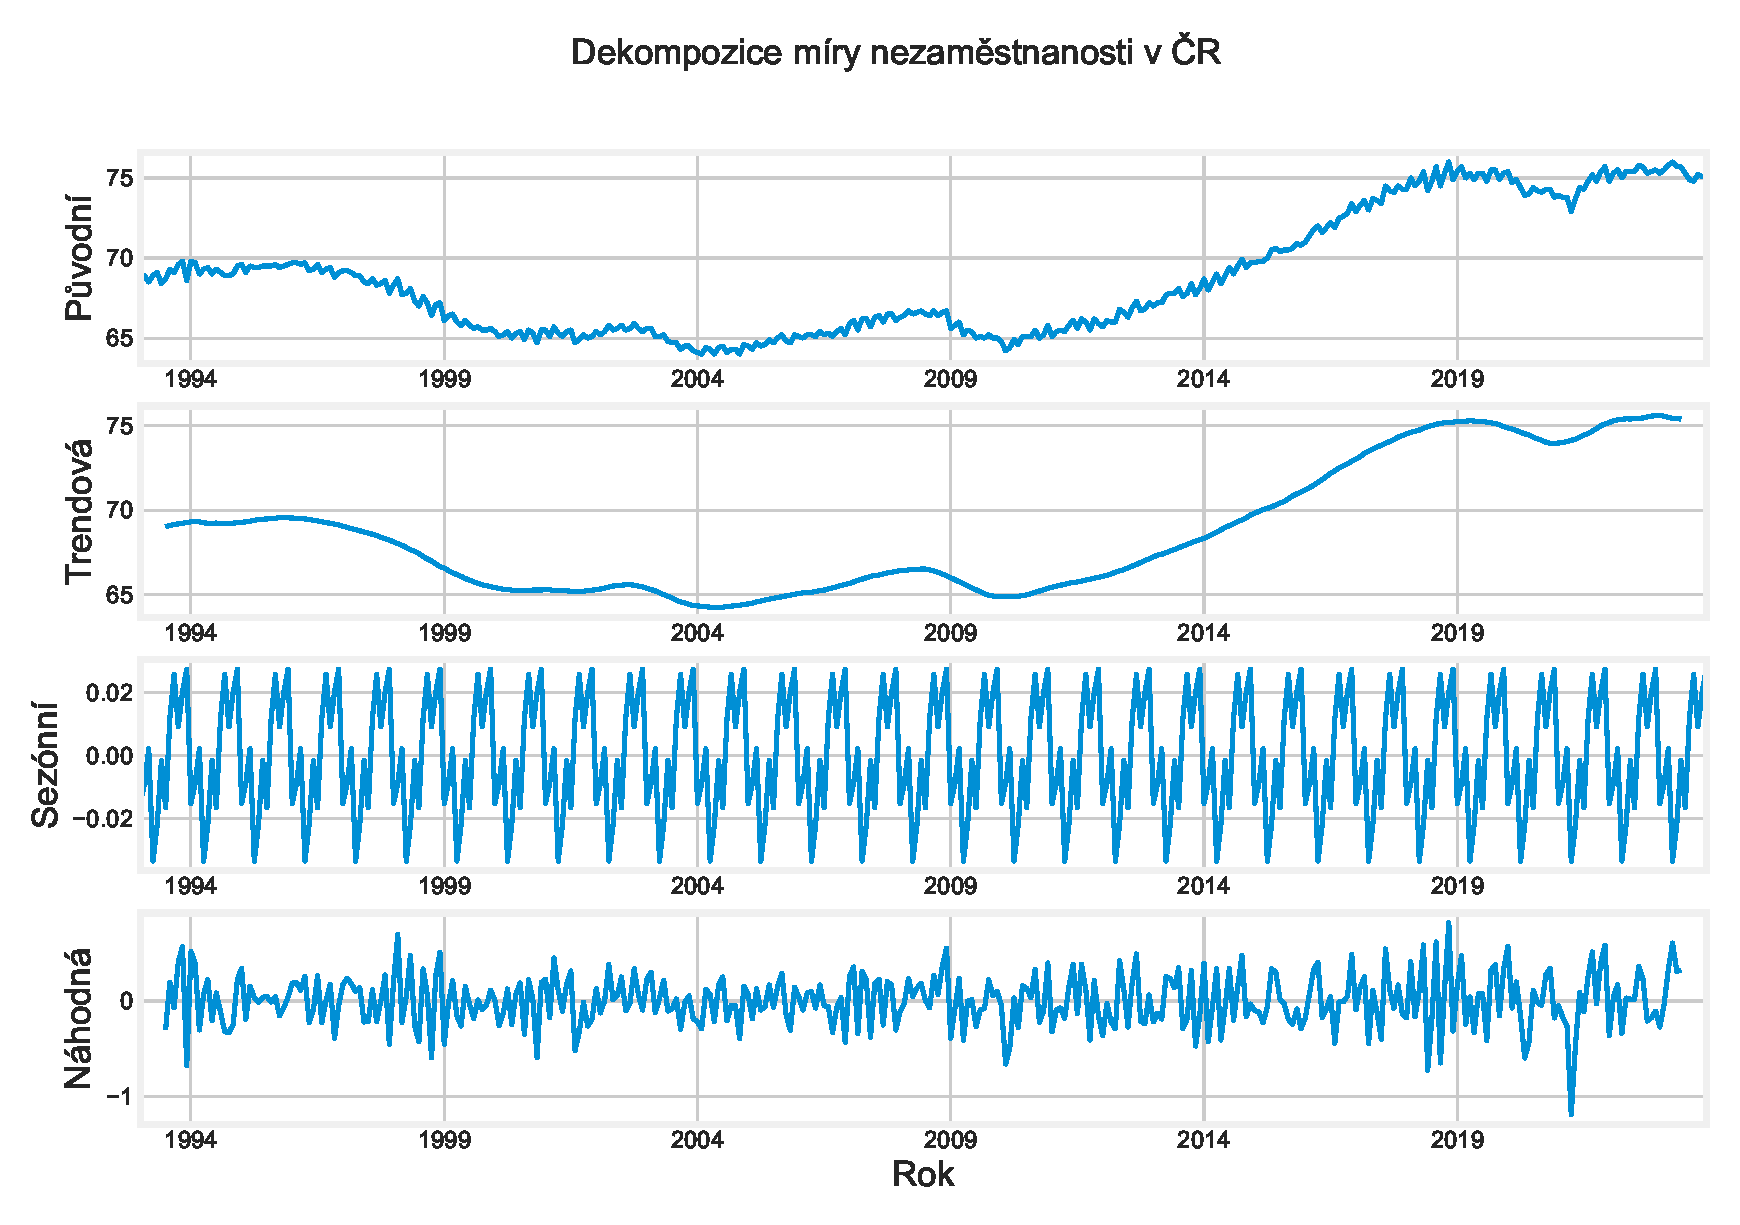
\includegraphics[width=0.8\textwidth]{pv_eg_03_classical_decomposition.eps}}%
	\caption{Klasická dekompozice s aditivním modelem pro data s měsíčními záznamy o míře nezaměstnanosti v ČR od roku 1993 }
	\label{fig:my_graph}
\end{figure}

V náhodné komponentě nám zbyla časová řada po odstranění trend-cyklické a sezónní komponenty. Někdy se jí místo náhodná říká detrendizovaná komponenta. V tomto případě model byl aditivní, tedy odstranění proběhlo jako $\epsilon_t = x_t - T_t - S_t$, pro multiplikativní model by vztah vypadal jako $\epsilon_t = \frac{x_t}{T_tS_t}$

Z pohledu na graf výše je vidět, že řada má nějaký trend i sezónnost. Na grafu náhodné komponenty lze zaznamenat několik vysokých výkyvů. V roce 2008 náhodná komponenta ukázala výrazný nárůst nezaměstnanosti, který nelze vysvětlit trendem, ani cyklickou složkou. (V tomto roce začala tzv. Velká recese).

 Další je vidět v roce 2019, kde Česká Republika měla silnou rostoucí ekonomiku. Hned po roce 2019 je vidět další výkyv, tentokrát negativní, způsobený pandemií.

%No to asi ne%
\chapter{Průzkum současných trendů v oblasti prediktivních metod}
V současné době s rostoucím objemem sbíraných dat se stále více organizací zaměřuje na prediktivní modelování. Díky dnešním výkonným výpočetním technologiím je možné zužitkovat nasbíraná data a využít metody strojového učení pro přesné predikce a odhad budoucích trendů.

Tato kapitola si klade za cíl provést rešerši aktuálně používaných metod pro predikce. Výstupem by měl být výběr několika metod a jejich následná aplikace na datech o spotřebě.

\section{Regresní analýza}
V oblasti předpovědí spotřeby energie lze často najít modely, které byly vytvořeny pomocí modelování spotřeby energie touto technikou (nebo její podmnožinou). Jeden z důvodu, proč se používají je jednoduchost použití a interpretace.

Regresní model popisuje vztah mezi jednou nebo více nezávislými proměnnými a jednou závislou proměnnou. Cílem regresní analýzy je najít funkční vztah mezi závislými a nezávislými proměnnými, který je potom použít k predikci hodnoty závislé proměnné na základě hodnot nezávislých proměnných.

Regresní model s více než jednou proměnnou se zapisuje jako

\begin{equation}
	y = \beta_0 + \beta_1x_1 + \beta_2x_2 + ... + \beta_px_p +  \epsilon
\end{equation}

kde $y$ je výstupní proměnná, $\epsilon$ chybový člen a $\beta_i$, i=0, 1, 2 ... p jsou regresní parametry.

Po získání regresních koeficientů je možné použít rovnici výše k predikci spojité hodnoty. Regresní koeficienty se dají odhadovat pomocí metody nejmenších čtverců. Tento postup spočívá v nalezení hodnot parametrů $\beta$ takových, aby součet čtverců rozdílů mezi predikovanými hodnotami výstupní proměnné y a skutečnými hodnotami byl co nejmenší.  \cite{hanousek1992moderni}

Regresní analýza neříká nic o tom, jaký je mechanismus, kterým jsou tyto vztahy vysvětleny. To znamená, že regresní analýza může být velmi užitečným nástrojem pro předpovídání budoucích hodnot, ale nemůže sloužit jako nástroj pro vysvětlování příčin.

% Tohle asi hodím dopíči
\subsection{Regresní modely}
Existuje několik druhů regresních modelů, jenž se používají v různých případech v závislosti na povaze dat a cíle analýzy. Jedním z nejprimitivnějších modelů je lineární regrese, zpravidla se používá jako validační model při práci s velkými a komplexními datovými sadami, jelikož nedosáhne stejných výsledků jako pokročilejší metody. Její princip spočívá v prokládání dat přímkou a hledáním parametrů dané přímky, aby co nejlépe modelovaly vztah mezi proměnnými.

Často se stává, že datové sady mají mnoho různých parametrů. Například v práci bude využita datová sada, která obsahuje informace o počasí v určitých časových intervalech. Ukáže se, že některé parametry mezi sebou vysoce korelují a to může mít vliv na stabilitu regresního modelu. V praxi proto lze pro predikci spotřeby najít ještě jeden užitečný regresní model s názvem ridge (hřebenový). Tento model přistupuje k problému vysoké korelace tím, že zahrnuje další regularizační parametr do regresního modelu, který penalizuje vysoké koeficienty (ty co spolu korelují).

\section{ARIMA}
ARIMA model je pravděpodobně mezi nejznámějšími a nejpoužívanějšími modely pro predikci časových řad. \ref{tohlenekdedohledat} Klíčové prvky modelu spojují;	 autoregresi AR($p$), integraci I($d$) a klouzavý průměr MA($q$) \ref{neco}. Samotná rovnice ARIMA modelu je tedy kombinací stacionarizovaného autoregresního modelu a k tomu přidaný model s klouzavým průměrem.
\subsection{Autoregresivní model}
Autoregresní model lze popsat jako funkci, jenž vrací predikovanou hodnotu $x_t$ na základě svých předchozích hodnot $x_{t-1}, ...,  x_{t-p}$. Těmto hodnotám se říká zpožděné (lag) proměnné a slouží ke zvýšení přesnosti autoregresního modelu. 

Toho se dosahuje snižováním hodnoty $t$, která označuje počet kroků v časové řadě dat. Vyšší počet těchto kroků umožňuje modelu zachytit více předchozích předpovězených hodnot jako vstup. Například se dá rozšířit autoregresní model tak, aby zahrnoval předpovězenou teplotu za posledních 7 dní až po posledních 14 dní, což může přispět k přesnějším výsledkům. \ref{amazon} Obecně bychom mohli model zapsat jako funkci: 

\begin{equation}
	x_t = f(x_{t-1}, x_{t-2}, ..., x_{t-p}, \epsilon_t)
\end{equation}
kde $\epsilon_t$ je bílý šum, který platí pro data co mají průměr a variaci dat nulovou. Počet zpožděných proměnných určuje parametr $p$ v AR($p$).

Někdy se nehodí, aby veškeré zpožděné proměnné měly stejnou váhu. Model je připraven na použití vážených parametrů a díky tomu lépe reagovat na výkyvy v časové řadě. Výsledná rovnice pro autoregresní model s váženými parametry $\alpha$ bude vypadat následovně: 

\begin{equation}
	x_t =    \sum_{i=1}^{p}\alpha_ix_{t-i} + \alpha_0 + \epsilon_t
\end{equation}

kde $\alpha_0$  je výchozí konstantní bod pro predikce (může být nulový a tedy být zanedbán). 

\subsection{Model klouzavého průměru}
Ačkoliv model nese stejný název jako kapitola v dekompozici časových řad, nesmí se tyto dva pojmy zaměnit. V prvním případě se jedná o výpočet pro vyhlazení a získání trend-cyklické komponenty. 

V tomto případě se jedná o model, který používá pro předpovězení nové hodnoty $x_t$ předchozí hodnoty z náhodné komponenty $\epsilon_t, \epsilon_{t-1}, ..., \epsilon_{t-q}$. Počet těchto zpožděných hodnot ovlivňuje parametr $q$ v MA($q$). Stejně jako u autoregresního modelu i zde se počítá s váhami. Finální rovnice modelu se zapíše jako: 

\begin{equation}
	x_t =  \sum_{i=1}^{q}\alpha_i\epsilon_{t-i}
\end{equation}


\subsection{ARIMA model}
Pro analýzu časových řad se zpravidla vyžaduje stacionarita řady, ARIMA není výjimkou. Tato podmínka vyžaduje tedy stacionarizovat výše zmíněný autoregresní model pomocí diference. 

Pokud se spojí tedy AR model po diferenci s modelem klouzavého průměru obdržíme rovnici ARIMA modelu: 

\begin{equation}
 x_t =    \sum_{i=1}^{n}(\alpha_i \Delta x_{t-i}) + \sum_{i=1}^{n}(\alpha_i\epsilon_{t-i}) + \alpha_0 + \epsilon_t
\end{equation}

kde $x_t$ je nová hodnota. Odhad jednotlivých parametrů $p$ a $q$ je jedním z kroků používané Box-Jenkinsovy metody. \ref{nejaky-ref-na-box-jenkina} Tato metoda využívá dvě funkce. Autokorelační funkci využívá pro odhad zpožděných parametrů modelu klouzavého průměru a parciální autokorelační funkci pro odhad parametrů autoregresního modelu. Použití této metody bude ukázáno v praktické části této práce.


\section{Rozhodovací stromy}
Pro strom existuje mnoho analogií a jedna z analogií se dostala i do modelování. Rozhodovací stromy můžou pomoci jak s klasifikačními, tak i s regresními problémy. 

Jak název napovídá, při tvorbě rozhodovacího stromu je snaha rozdělit data na menší a jednodušší skupiny pomocí pravidel (segmentace dat), která se postupně aplikují na různé atributy dat. Cílem je vytvořit sadu pravidel, která umožní co nejpřesněji predikovat hodnotu požadované proměnné pro nově příchozí data.

Při tvorbě stromu se postupuje od shora dolů. V kořeni stromu je nutné zvolit jeden hlavní dělící parametr s nejvyšší schopností rozlišení dat, například "výška < 1.85.m" a dále se již větví na základě největšího poměrného \textit{informačního zisku} (založeno na výpočtu entropie).  \cite{Tomsik2016thesis}

Pro tvorbu těchto stromů existuje mnoho metod. Zpravidla založených na statistických metodách. Nejčastějšími zástupci těchto metod jsou algoritmy \textbf{gradientní boostované stromy}, CHAID, C5.0 či náhodné lesy. \cite{Tomsik2016thesis}

\begin{figure}[htbp]
	\centering
	\makebox[\textwidth][c]{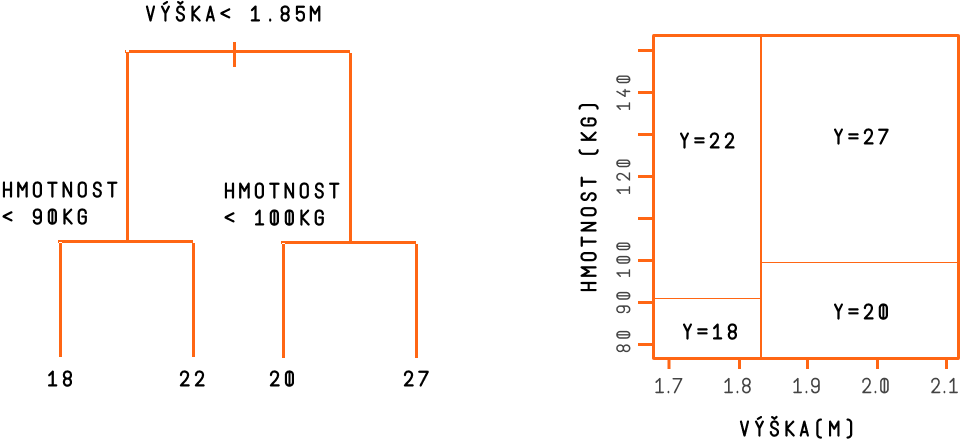
\includegraphics[width=0.7\textwidth]{trees.png}}%
	\caption{Ukázka rozhodovacího stromu}
	\label{fig:my_graph}
\end{figure}
\subsection{Gradientní boostované stromy}\label{xgboost_research}
Tato metoda je přesná a použitelná pro oba základní problémy, klasifikaci i regresi napříč různými odvětvími. Jelikož se tato práce zabývá predikcí spotřeby energie, což je spojitá veličina, budou prozkoumány možnosti regresního řešení problémů s pomocí GBT.

Hlavním úkolem boostování je sestavit z mnoha slabších modelů výrazně silnější model, takzvaně \textit{ensemble  model}. \cite{chen2016xgboost}

V každé iteraci se vytváří nový rozhodovací strom, který se zaměřuje na opravu chyb (reziduí) předchozího stromu. Tímto způsobem je postupně zlepšována přesnost predikce a minimalizována chybovost modelu. 

Mezi nejpopulárnější implementace GBT patří například XGBoost, LightGBM a CatBoost. Tyto implementace využívají různé optimalizace a techniky pro minimalizaci přeučení a maximalizaci přesnosti predikce.

Pro tuto práci byla zvolena implementace XGBoost v Pythonu pro svou přehlednou dokumentaci a jednoduchosti použití


\section{Neuronové sítě}
V poslední letech si neuronové sítě vydobyly své postavení na poli analýzy a predikci dat. Neuronové sítě fungují dobře v problematice predikce hodnot, kde nejsou známy matematické vzorce a předchozí znalosti o vztazích mezi vstupy a výstupy. Fungují dobře v této problematice díky svému původu a díky inspiraci v neurofyziologii lidského mozku.

Na první pohled to může vypadat, že neuronové sítě jsou novinka posledního století. Není tomu tak, je to pouze posunutím vývoje výkonného hardwaru kupředu. Neuronové sítě tu jsou již od 50. let, kdy Warren McCulloch a matematik Walter Pitts vydali publikaci, ve kterém modelovali zjednodušený model neuronu s elektrickým obvodem, jehož aktivační funkce byla pouze binární. \cite{mcculloch1943logical}

\begin{equation}
	y = \begin{dcases}
		1 & z \geq T \\
		0 & z < T
	\end{dcases}
\end{equation}

Autoři práce také ukázali, jak se dají sestrojit pomocí neuronu jednoduché logické funkce: 

\begin{figure}[htbp]
	\centering
	\makebox[\textwidth][c]{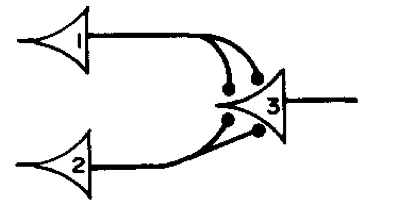
\includegraphics[width=0.3\textwidth]{disjunkce.png}}%
	\caption{Logický součet pomocí biologických neuronů}
	\label{fig:logic_or}
\end{figure}

Neuron označují jako $N$ s indexem $i$, který je uvnitř neuronu. V tom případě na obrázku výše lze vidět $N_3(t) = N_1(t-1) \vee N_2(t-1)$, což znamená, že se jedná o logický součet. \cite{mcculloch1943logical} Autoři v práci dále naznačili, jak se dají skládat tyto neurony do sítě. 

Toto položilo první základy na rozvoj neuronových sítí v roce 1957 Frankem Rosenblattem, který začal práci na perceptronu.
\newpage
\subsection{Perceptron}
Perceptron je nejjednodušší model dopředné neuronové sítě, který se skládá z jednoho jediného neuronu.

Perceptron přijímá na vstupu vektory $x_i$, ke kterým je přiřazena váha $w_i$. $b$ je potom práh (bias), jenž ovlivňuje nakolik musí být suma vah větší než 0, aby se perceptron aktivoval. \cite{martinpilatNN}. Aktivace neuronu se pak spočítá následovně:
\label{eq:activation_percep}
\begin{equation}
	z = \sum_{i=1}^{n} w_xx_i + b
\end{equation}

A samotný výstup perceptronu (neuronu) $Z$, kde oproti jednoduchému neuronu nemusí být pouze binární přenosová funkce, ale libovolná přenosová funkce (zpravidla skoková nebo sigmoidální pro jeden perceptron) \cite{martinpilatNN} se spočítá jako:

\begin{equation}
	Z = H(z)
\end{equation}
kde
\begin{equation}
	H(z) = \begin{dcases}
		1 & f(z) \geq 0 \\
		0 & f(z) < 0
	\end{dcases}
\end{equation}

Učení perceptronu probíhá jednoduše. Na vstup se přivede $(x,y)$ z trénovací sady (kde $x$ jsou příznaky a $y$ požadované výstupy) a aktualizují se váhy perceptronu dle rovnice:

\begin{equation}\label{eq:learning_percep}
	w_{n,i} = w_i + r(y_i-Z_i)x_n
\end{equation}
kde $r$ je parametr učení, který určuje, jak rychle se mění váha a kde $n$ je n-tý vstup.  

Důležitým poznatkem je to, že tento perceptronový algoritmus je jednoduchý a efektivní pro řešení lineárně rozdělitelných problémů, ale není schopný řešit problémy, které nejsou lineárně rozdělitelné. Například funkci XOR, která se chová nelineárně, již tímto způsobem nelze vyřešit. To vedlo k rozšíření této oblastí a vznikly tak vícevrstvé perceptrony, kde se pro učení používá algoritmus zpětného šíření.




\subsection{Vícevrstvé perceptrony}
Vícevrstvé perceptrony mají na rozdíl od perceptronu ještě skryté vrstvy, které se nachází mezi vstupní a výstupní vrstvou. Skrytých vrstev může být více nebo jenom jedna, to už záleží na volbě programátora a na typu problému. Neuronové sítě s jednou vrstvou se nazývají mělké. Sítě s více skrytými vrstvami se nazývají hluboké sítě. V souvislosti s vícevrstvými perceptrony se mluví také o dopředné síti (feedforward). Vstupní vektor dat $I = (x,y)$ jde do skrytých vrstev $H$ a poté na výstup $Y$. Vektor hodnot z výstupní vrstvy označíme jako $Y$. 

\newpage
Výstup $Y$ poté získáme pomocí rovnice níže 

\begin{equation}
	H_i = \sigma(w_{ni} \cdot I_n + b_i)
\end{equation}


\begin{equation}
	Y = \sigma(w_{ij} \cdot H + b_{out})
\end{equation}

kde $\sigma$ označuje přenosovou funkci a $w_{ni}$ váhu spojení mezi n-tým vstupním a í-tým výstupním neuronem.

Ve více vrstvých sítích se používají jiné přenosové funkce než v samostatném perceptronu. V současnosti vyčnívá jedna velmi používaná funkce ReLU (rectified linear unit), která se definuje jako:

\begin{equation}
	Relu(z) = max(0, z)
\end{equation}

a používá se především ve skrytých vrstvách. \cite{brownlee2019gentle} Na výstupní vrstvě je zpravidla funkce softmax, definovaná jako:

\begin{equation}
	\sigma(z_i) = \frac{e^{z_{i}}}{\sum_{j=1}^n e^{z_{j}}} \ \ \ pro\ i=1,2,\dots,n
\end{equation}

Pro trénování pak již nelze použít klasický perceptronový algoritmus (viz \ref{eq:learning_percep}). Nejčastěji se používá algoritmus zpětného šíření (back-propagation).

Při použití algoritmu zpětného šíření se výstupní chyba sítě propaguje zpět k vstupní vrstvě, přičemž se upravují váhy všech spojů v síti tak, aby se minimalizovala tato chyba. Tento proces se opakuje v průběhu několika iterací (epoch).

V kontextu práce by se dalo psát o optimalizačních metodách, chybových funkcích a o tom jak jednotlivé vrstvy fungují, ale to je nad rámec této rešerše. Pro tuto práci je důležité zmínit \textit{long short-term memory networks}, které vycházejí z rekurentních sítí, které budou popsány v další kapitole.


\subsection{Rekurentní neuronové sítě}
Zatím byly zmíněny pouze sítě, kde výstup závisí pouze na aktuálním vstupu. V této práci je vstupem časová řada popisující spotřebu energie, která nezávisí pouze na aktuálním stavu a ke správnému výstupu by bylo vhodné zahrnout data předchozí.

Rekurentní sítě toto umožňují tím, že obsahují zpětná spojení, která fungují jako vnitřní stav (paměť). Nejjednodušší příklad rekurentní neuronové sítě může být síť, co má jeden vstup, výstup a jeden neuron ve skryté vrstvě. Když tento neuron bude mít spojení sám do sebe, tak při předložení vstupu neuron dostane kromě vstupu ještě aktivaci $h_{(t-1)}$ z minulého vstupu. Nejnázornější je ukázat jak se změní výpočet výstupu z neuronu, když se přidají zpětná spojení.


\begin{equation}
	h_t = \sigma(w_{hh}h_{t-1} + w_{xh}x_t)
\end{equation}

kde $h_t$ je aktuální stav neuronu, $x_t$ je vstupní sekvence v čase $t$, $w_{hh}$ váha rekurentního neuronu a $w_{xh}$ váha vstupního neuronu. Zásadní změna oproti aktivaci v jednoduchém perceptronu (viz \ref{eq:activation_percep})  je, že aktivace $h_t$ závisí i na předchozí aktivaci neuronu $h_{t-1}$.

Trénování sítě probíhá opět algoritmem zpětného šíření, avšak lehce modifikovaným. Jmenuje se algoritmus zpětného šíření v čase (backpropagation throguh time). S trénováním rekurentních sítí se můžou vyskytnout dva problémy, díky tomu jak se zpětné šíření počítá. \cite{martinpilatRNN} Gradient se vždy násobí váhou. Pokud je toto rekurentní váha, tak se opakovaně násobí stejnou hodnotou. V případě, že tato hodnota bude větší než 1, dojde k problému explodujících gradientů, kdy hodnoty nekontrolovatelně rostou. V opačném případě, kdy je hodnota menší než 0, tak dochází k problému s mizejícími gradienty.

Jedno z možných řešení je použít další typ sítě. Tento typ sítě se jmenuje long-short term memory network a problém řeší tak, že rekurentní váha se zafixuje na hodnotu 1 a práce se stavem se provádí explicitně.



\subsection{Long short-term memory networks}\label{nn-lstm}
LSTM sítě jsou speciální druh rekurentních sítí, které dokáží zpracovat  bez problému jednorozměrné signály a časové řady. Klíčovým prvkem těchto sítí jsou tzv. LSTM buňky, které nahrazují každý neuron. 

Tyto buňky se skládají typicky z pěti prvků. Mezi tyto prvky patří input gate, forget gate, cell gate, output gate a samotná cell, která je jako aktuální stav ovlivňovaná vyjmenovanými prvky.

\begin{figure}[htbp]
	\centering
	\makebox[\textwidth][c]{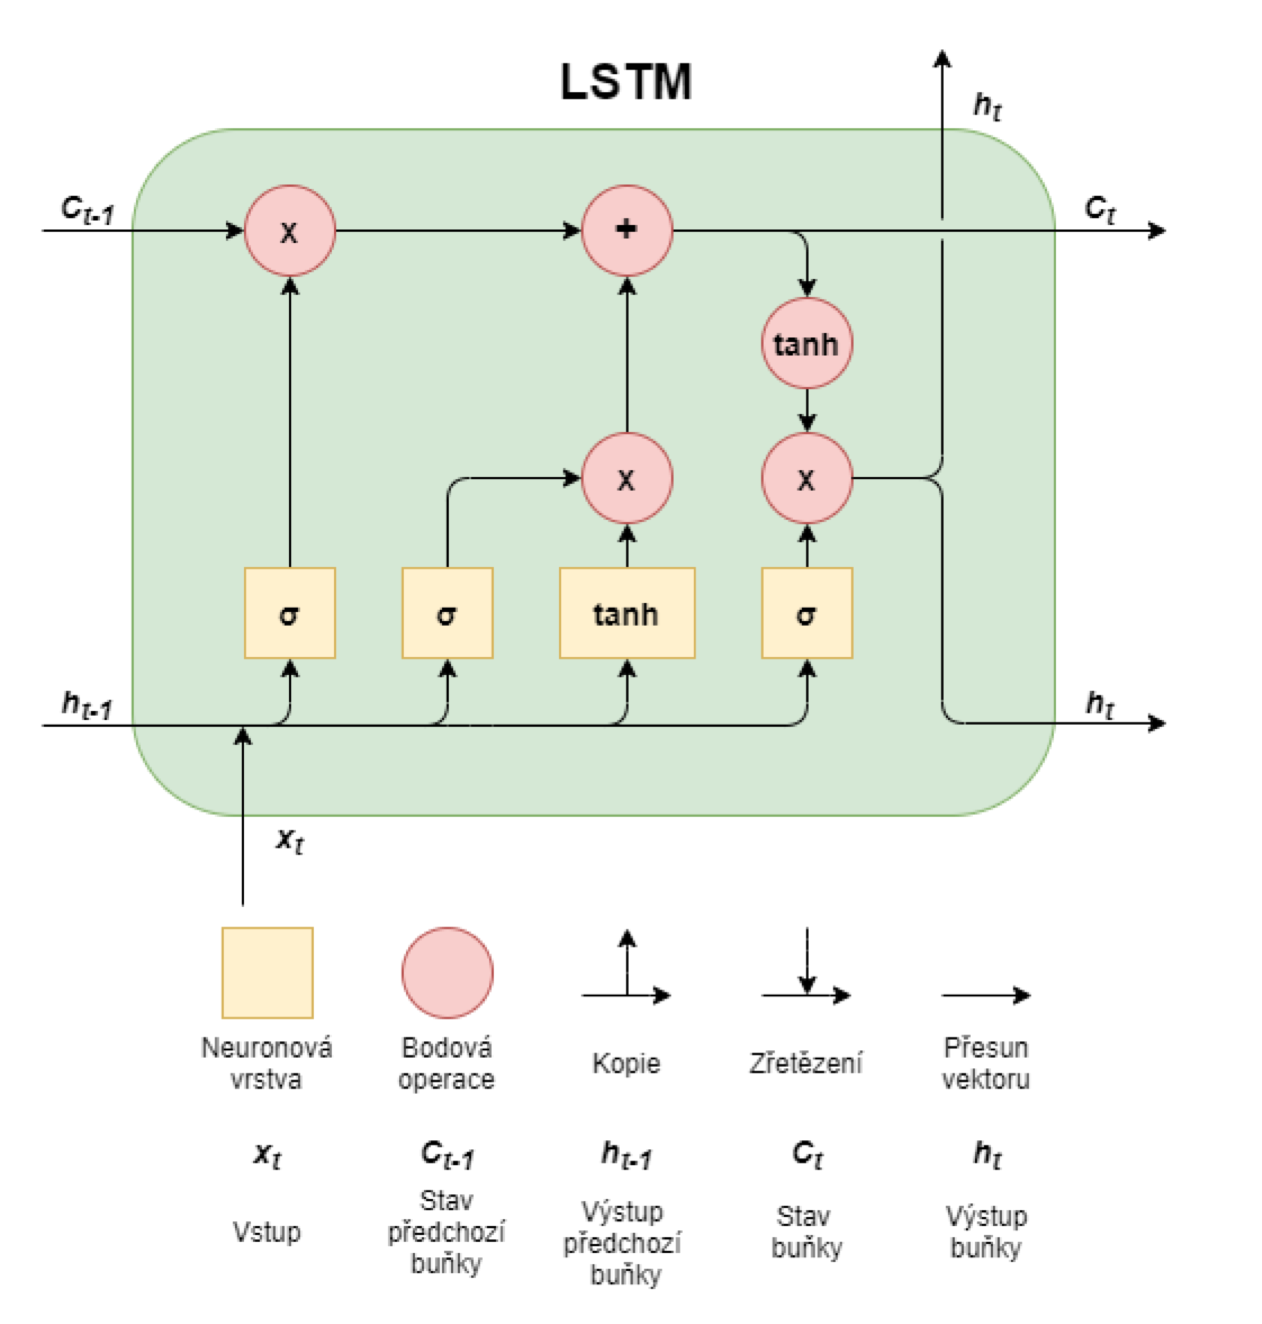
\includegraphics[width=0.55\textwidth]{lstm_cell.png}}%
	\caption{Jedna buňka LSTM sítě (převzato a přeloženo z \cite{colah})}
	\label{fig:my_graph}
\end{figure}

LSTM mají řešit problém klasických RNN a to explodující a mizející gradienty. Problém je řešen tak, že přenos informací mezi časovým krokem probíhá pomocí stavu, s kterým není spojená žádná váha a díky tomu se při propagaci chyby dá vyhnout násobení, které by mohlo vyvolat tento problém. Díky této vlastnosti si LSTM sítě umí zapamatovat delší posloupnosti vstupů než základní rekurentní neuronové sítě.

Při rešerši autor práce narazil také na kombinaci více sítí v jednu. Autoři jedné z prací zabývající se predikcí spotřeby energie v domácnosti \cite{cnn-bi-lstm}	 využívají například Bi-LSTM (obousměrná LSTM síť), CNN-LSTM (konvoluční neuronová síť s LSTM sítí) a kombinaci všeho - CNN-Bi-LSTM síť.

Kromě LSTM sítě existuje ještě její zjednodušená verze, které chybí output gate. Nazývá se gated recurrent unit (GRU) a v některých případech dosahuje vyšších přesností než LSTM, hlavně na menších datových sadách a převážně v oblast zpracování přirozeného jazyka. \cite{kynych2018vyuziti}

\section{Konvoluční neuronové sítě}
Již z názvu vyplývá, že konvoluční neuronové sítě (CNN) jsou podmnožinou neuronových sítí. Zpravidla se vyznačují využitím konvolučních a poolingových vrstev. Tyto vrstvy umožňují efektivnější zpracování velkých vstupů s menším počtem potřebných parametrů nežli klasická neuronová síť. 

Toto je jeden z důvodu, proč je tento typ sítí široce využíván v oblasti počítačového vidění. \ref{springer}

V porovnání s klasickými metodami, jako jsou autoregresivní modely nebo regresní metody, mohou konvoluční neuronové sítě poskytovat lepší výsledky při zachycování nelineárních a lokálních vzorů v datech. Tyto vlastnosti mohou být klíčovými faktory pro úspěšnou predikci profilů spotřeby energie.

Typická konvoluční neuronová síť se tedy skládá z několika klíčových prvků. Hlavním stavebním kamenem je operace zvaná konvoluce, ta se využívá v ostatních vrstvách jako jsou konvoluční a poolingové vrstvy, které se starají o extrakci příznaků.

\subsection{Konvoluční vrstva}
V této vrstvě se děje matematická operace zvaná konvoluce. Základem je takzvané konvoluční jádro, což je obyčejná matice o rozměrech $m$ a $n$. V oblasti počítačového vidění se toto konvoluční jádro postupně přikládá na vstupní obrazovou matici, poté se pronásobí na sobě ležící prvky a jejich suma se zapíše do výstupní matice. Následuje posunutí jádra o definovaný krok a tento proces se opakuje. Konvoluce s jednotkovým krokem se dá tedy zapsat jako:

\begin{equation}
    y_{i,j} = \sum_{a = 1}^{m} \sum_{b = 1}^{n} f_{a,b}x_{i+a,j+b}
\end{equation}

kde $f_{i,j}$ jsou prvky konvolučního jádra, $x_{i,j}$ prvky vstupní matice a $y_{i,j}$ prvky výstupní matice. zjednodušeně se konvoluce zapisuje jako:
\begin{equation}
    Y = X \otimes F
\end{equation}
kde $F$ je konvoluční jádro, $X$ vstupní matice a $Y$ výstupní matice.

Tato vrstva dokáže extrahovat lokální charakteristiky vstupní matice (obrazu) při schopnosti zachovat informaci o jejich pozici. Mezi tyto extrahované charakteristiky můžou patřit rohy či barvy obrazu.\ref{cvut}


\begin{figure}[htbp]
	\centering
	\makebox[\textwidth][c]{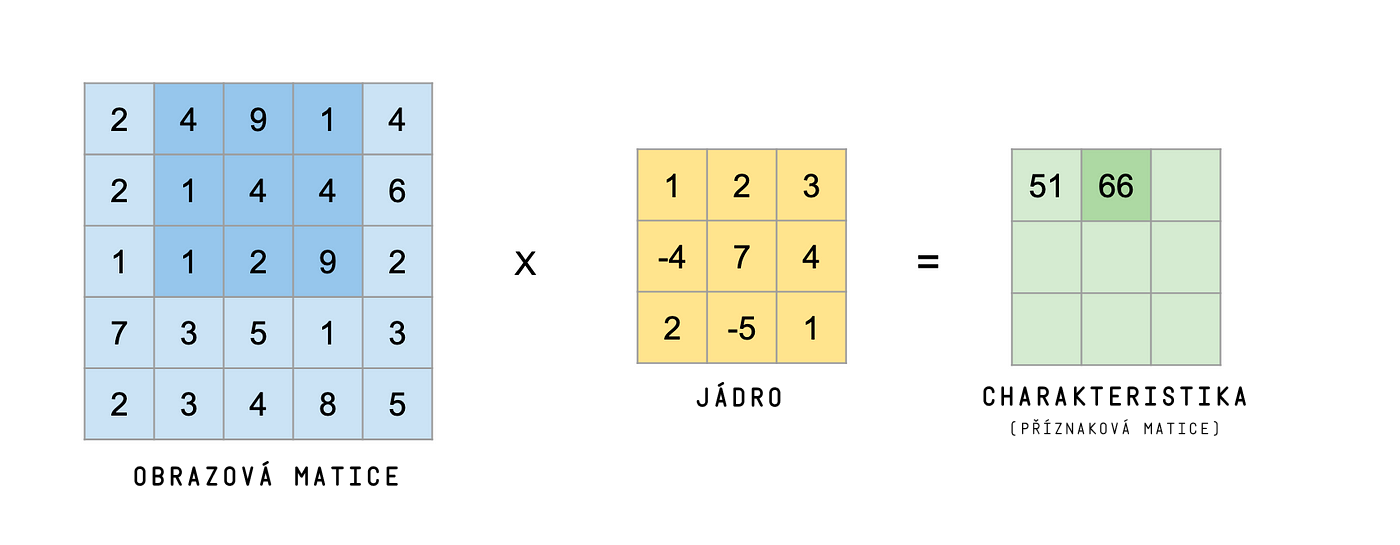
\includegraphics[width=0.8\textwidth]{convolution.png}}%
	\caption{Ukázka extrakce charakteristiky z obrazu pomocí konvoluce }
	\label{fig:nezamestnanost}
\end{figure}

Opakem konvoluční vrstvy je dekonvoluční vrstva, která provádí inverzní operaci ke konvoluci. 

\subsection{Poolingová vrstva}
Tato vrstva je vždy přímo za konvoluční vrstvou a slouží k snížení velikosti vstupů z předchozí vrstvy, což má za následek snížení výpočetní náročnosti (snížením počtu parametrů) a zlepšení distribuce informace.

Nejčastěji lze potkat maxpool vrstvu, která má tři základní parametry. Velikost jádra $m$ a $n$, krok na ose x $h$ a krok $v$ po ose y. Vrstva vždy vybere maximální hodnotu v daném překrytí obrazu jádrem a vloží její výstup do výstupní matice a posune se dále.

\begin{figure}[htbp]
	\centering
	\makebox[\textwidth][c]{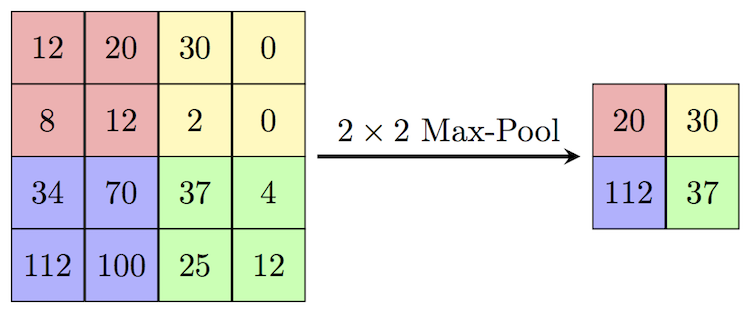
\includegraphics[width=0.4\textwidth]{maxpool.png}}%
	\caption{Ukázka maxpool operace s krokem $h=2$ a $v=2$ }
	\label{fig:nezamestnanost}
\end{figure}

\subsection{CNN-LSTM}\label{cnn-lstm-teorie}
Pro analýzu časových řad se využívá hybridního modelu, který je spojením konvoluční neuronové sítě a LSTM sítě. Tato metoda se snaží využít silných stránek obou modelů. 

Konvoluční vrstvy v síti jsou schopné extrahovat lokální vzorce chování spotřeby energie. V praxi to znamená, že konvoluční vrstvy mohou identifikovat specifické charakteristiky, jako jsou špičky či útlumy, což je klíčové pro porozumění dynamiky spotřeby energie v čase. 

Přidáním LSTM sítě lze zachytit na druhou stranu dlouhodobé vzorce chování v časové řadě, díky své rekurentní architektuře.
 Například mohou úspěšně identifikovat sezónní trendy, které se opakují v pravidelných intervalech, a analyzovat dlouhodobé změny v chování spotřeby, což může být zásadní zejména v oblasti plánování a optimalizace energie. 

V předchozích kapitolách bylo uvedeno, že CNN se většinou používá pro 2D obrazová data. Časové řady jsou  jednodimenzionální, takže klasická 2D konvoluční vrstva nemůže být využita.

Tomuto problému se dá vyhnout pomocí 1D konvoluční vrstvy, kde se dělá konvoluce pro jednu dimenzi. \ref{neco}

Druhý způsob je provést časově frekvenční transformaci signálu. \ref{ieee} Výsledkem této transformace je rozmístění frekvencí signálu v čase. Zpravidla se jedná o spektogram pomocí Fourierovy transformace a nebo se může jednat o vlnkovou transformaci, kterou zobrazuje scalogram.


\chapter{Aplikace vybraných metod}
V této kapitole bude popsán způsob aplikace metod z rešeršní části této práce. Jednotlivé metody byly vybrány na základě dostupnosti knihoven a očekávaných výsledků.

První zvolená metoda jsou rozhodovací stromy, pro konkrétní implementaci byly zvoleny gradientní boostované stromy, pro které je dostupná knihovna XGBoost. Jako druhou metodou byl zvolen klasický statistický přístup, konkrétně statistický model ARIMA, jež se standardně používá pro predikci časových řad. Další metody jsou postavené na rekurentních neuronových sítích, tedy výše popisovaná LSTM síť a kombinace konvoluční neuronově sítě s LSTM sítí. Zde bude využito bohaté knihovny Tensorflow od společnosti Google

Před samotnou aplikací těchto metod bude kladen důraz na základní datovou analýzu, která má klíčový význam při identifikaci optimálních parametrů pro finální modely. Tato analýza umožní lépe porozumět datům, identifikovat vzorce a trendy ve spotřebě elektrické energie a získat ucelenou představu o nejdůležitějších faktorech ovlivňujících spotřebu.

Výsledkem této kapitoly budou natrénované modely, jež budou využívány k predikci budoucích hodnot spotřeby elektrické energie pomocí vybraných metod. Jako jedno z rozšíření této práce v budoucnu je integrace těchto modelů do informačního systému NEO.  

Nakonec budou tyto modely podrobeny důkladnému hodnocení založenému na metrikách přesnosti, které jsou uvedeny v kapitole \ref{section:error-matrix}. Vyhodnocení na základě těchto metrik bude klíčovým krokem při posuzování celkové úspěšnosti modelů a pomůže identifikovat případné oblasti, které vyžadují zdokonalení. Vyhodnocení povede také k informovanému rozhodování o jejich budoucí integraci v informačním systému NEO.

V rámci implementace byl využit programovací jazyk Python a základní statistické knihovny, jako jsou numpy, pandas a statsmodels, spolu s knihovnami specializovanými pro strojové učení, jako jsou Keras, Scikit-learn a další. Tato kombinace nástrojů poskytla robustní prostředí pro vývoj a testování predikčních modelů.

\newpage
\section{Zdroj dat}
V práci byly využity dva klíčové zdroje dat. První ze zdrojů je veřejný a jedná se o kolekci 5567 domácností, které se zúčastnili projektu UK Power Networks vedené společností Low Carbon London mezi roky 2011 a 2014. 

Cílem tohoto projektu byla inovace distribuční soustavy v Londýně a zvýšení využívání nízkouhlíkových technologií pro vytápění. V průběhu počáteční fáze projektu byly domácnosti vybaveny chytrými elektroměry, a následně byl spolu s příslušnou studií zveřejněn vzorek dat \cite{londondata}

Naměřená data jsou dostupná v půlhodinových intervalech a obsahují informace o spotřebě v kWh, unikátní identifikátor domácnosti (LCLid) a časové razítko. Celá datová sada má rozsah přes 10 GB a obsahuje více než 160 milionů záznamů.

Struktura datové sady s energetickou spotřebou v domácnostech v Londýně je detailně popsána následovně:
 \renewcommand{\arraystretch}{1.1}
\begin{table}[!ht]
	\centering
	\caption{Struktura datové sady se spotřebou v domácnostech (Londýn)}
	\begin{tabularx}{\linewidth}{ll}
		\hline
		\textbf{Sloupec} & \textbf{Popis} \\ \hline
		LCLid & Unikátní identifikátor domácnosti \\ 
		tstp & Časové razítko ve formátu YYYY-MM-DD hh:mm:ss \\ 
		energy(kWh/hh) & Spotřebovaná energie v kWh \\ 
		\hline
	\end{tabularx}
\end{table}

Pro tvorbu robustnějších modelů a podrobnějších analýz byl také zveřejněn datový soubor s hodinovými rozlišením o počasí získaný z \textit{Dark Sky} API. Tato sada má následující strukturu:


\begin{table}[!ht]
	\centering
	\caption{Struktura datové sady s počasím pro Londýn}
	\label{weather_dataset}
	\begin{tabularx}{\linewidth}{lX}
		\hline
		\textbf{Sloupec} & \textbf{Popis} \\ \hline
		visibility & Maximální viditelnost \\ 
		windBearing & Směr, ze kterého fouká vítr \\ 
		temperature & Skutečná teplota ve stupních Celsia \\ 
		time & Časové razítko ve formátu YYYY-MM-DD hh:mm:ss	 \\ 
		dewPoint & Rosný bod \\ 
		pressure & Aktuální atmosférický tlak měřený v hektopascálech. \\ 
		apparentTemperature & Pocitová teplota, která je kombinací vlhkosti a reálné teploty \\ 
		windSpeed & Rychlost větru měřená v km/h \\ 
		precipType & Typ srážky (sníh nebo déšť) \\
		icon & Název ikony signalizující oblačnost, slunečno, atd.  \\ 
		\hline
	\end{tabularx}
\end{table}


Pro účely této práce je nezbytné provést transformaci dat o počasí, aby byla dosažena konzistence a kompatibilita s datovou sadou pro Londýn. Tato transformace spočívá v rozdělení časových údajů o počasí do intervalů po půl hodinách. Bez této transformace by nebylo možné využít datovou sadu pro Londýn v kombinaci s daty o počasí, aniž by se neztratila informace o měřené spotřebě.

V dalším kroku je nezbytné provést analýzu klíčových sloupců datové sady o počasí, aby bylo dosaženo přesnějších výsledků. Předpokládá se, že některé sloupce, například sloupec \textit{icon}, nemají signifikantní vliv na určení spotřeby energie. Tato analýza umožní identifikovat klíčové proměnné, které mají významný dopad na spotřebu energie, a tím zlepšit přesnost modelu.

Druhý zdroj dat, který je využíván, již není veřejně dostupný. Jedná se o komerční data, která jsou získávána společností Albistech s.r.o. Autor práce se jako zaměstnanec podílí na vývoji informačního systému NEO, který umožňuje komplexní sbírání dat získaných při měření v uzlových bodech distribuční soustavy. Systém NEO následně tato data zpracovává a poskytuje užitečné informace a přehledy.

Pro tuto práci byla zvolena lokální distribuční soustava, kterou provozuje zákazník LDEnergy. Náhodně bylo zvoleno několik odběrných míst v Brně a byly dohledány identifikátory příslušných elektroměrů. Všechna získaná data byla anonymizována a obsahují pouze časová razítka a naměřenou spotřebu v kWh s čtvrthodinovým rozlišením.


\begin{table}[!ht]
	\centering
	\caption{Struktura datové sady se spotřebou v domácnosti (Brno)}
	\label{structure-brno}
	\begin{tabularx}{\linewidth}{ll}
		\hline
		\textbf{Sloupec} & \textbf{Popis} \\ \hline
		wstime & Časové razítko ve formátu ddddd,sssss \\ 
		value & Spotřebovaná energie v kWh \\ 
		\hline
	\end{tabularx}
\end{table}

Struktura datové sady se spotřebou v domácnosti v Brně je popsána v tabulce \ref{structure-brno}, kde sloupec "wstime" reprezentuje takzvaný horolog. Sloupec "value" udává spotřebovanou energii v kWh.

Pro získání tohoto zdroje dat bylo nutné se seznámit s proprietární databázovou platformou IRIS od společnosti Intersystems, což zahrnuje pokročilejší orientaci v specifických prostředcích této platformy. Tato znalost byla nezbytná pro úspěšné zpracování a interpretaci dat v této práci.


\newpage
\subsection{IRIS Data Platform}
IRIS je vysoce výkonná multimodelová databáze, která se vyvinula z databáze jménem Caché, vytvořené společností Intersystems. Tato databáze, díky svým unikátním vlastnostem a širokým možnostem integrace, nachází své uplatnění zejména ve zdravotnickém a finančním sektoru, kde je potřeba pracovat s velkými a zároveň různorodými daty.

Klíčovou součástí celého ekosystému IRIS je modul, který se stará o ukládání dat, co mají být persistentně uložena (storage engine). Data jsou uspořádána v multidimenzionálních polích nazývaných "globály", které si lze představit jako hierarchickou strukturu ve formě stromu. Globály jsou řídká pole a databáze zde udržuje pouze tolik položek, kolik je prvků. To má za následek výrazně nižší hardwarové nároky oproti systému s relačními databázemi. 

Díky skvělé implementaci se dají s globály tvořit komplexní struktury, které mohou čítat několik stovek gigabajtů, a i přesto mít minimální odezvu na čtení a zápis dat. \cite{irisPlatform} Globály, také podporují transakce, mechanismy pro žurnálování a replikaci dat. Data jsou nepřetržitě k dispozici  objektovým přístupem, pomocí SQL či pomocí přímého přístupu do globálu. Její hlavní výhodou na rozdíl od jiných platforem, je ta, že data se uloží jednou a dále se k nim může přistoupit libovolným způsobem, aniž by bylo nutné provádět duplikaci dat nebo například object-to-relational-mapping. \cite{irisPlatform} Tato flexibilita dává vývojářům a datovým modelářům možnost zvolit optimální přístup nebo kombinaci přístupů, aby byla zajištěna maximální efektivita bez zbytečné komplexity.

K datům uloženým v IRIS je možné přistoupit několika způsoby. Prvním způsobem je použití jazyka Objectscript, který pohání celou datovou platformu IRIS. Tento jazyk umožňuje psát aplikační logiku, kterou následně platforma vystaví prostřednictvím REST API pro komunikaci.

Druhým možným přístupem je využití nativního rozhraní, které IRIS nabízí. V současné době poskytuje společnost InterSystems rozhraní pro Javu, .NET, Node.js a Python.\cite{irisPlatform} Pro tuto práci hraje klíčovou roli Python rozhraní, které umožňuje vytvářet aplikační logiku přímo v Pythonu nebo volat již existující logiku napsanou v Objectscriptu na straně IRIS.

Pro samotné získání dat k analýze byla v Objectscriptu vytvořena metoda \textit{GetData}, která přijímá identifikátor elektroměru jako parametr a vrací seznam časových razítek a hodnot elektroměrů od počátku zapojení, dle struktury zmíněné v tabulce \ref{structure-brno}. Při implementaci této metody bylo nutné pochopit komplexní strukturu několika globálů, provést iteraci přes globály a vhodným způsobem tato data vrátit. 

V Pythonu je poté pomocí nativního rozhraní metoda pro získání dat spuštěna a následně jsou data uložena do JSON souboru s příslušným identifikátorem a časovým razítkem pro další zpracování.  



\section{Explorační analýza dat a jejich příprava}
Jeden z mnoha klíčových bodů úspěšného projektu, jenž využívá metody strojového učení, je provést explorační analýzu dat (dále již jen EDA z Exploratory Data Analysis). Při provádění této analýzy se zkoumají předběžně vlastnosti dané datového sady. Před použitím metod strojového učení je vhodné znát vlastnosti, charakteristiku a jednotlivé závislosti mezi atributy, které budou zkoumány. Porozumění datům dokáže odhalit skryté vzorce, které nejsou na první pohled vidět.

Zpravidla se k analýze používá statistických nástrojů, které analytikům pomáhají vizualizovat závislosti a chování dat. Nejčastěji se k vizualizaci využívají krabicové grafy (box plot), histogramy nebo třeba teplotní mapy (heat mapy). 

Při analýze je kladen důraz na snížení dimenze dat či na odhalování atributů, co nesou signifikantnější informaci než ostatní atributy. K tomu bude v následující kapitole sloužit analýza hlavních komponent (Principal Component Analysis, PCA). 

Je též důležité věnovat pozornost identifikaci odlehlých hodnot (outlierů) v datech. Odlehlé hodnoty mohou výrazně ovlivnit výsledky analýzy či modelování, a tím měnit celkový obraz datové sady. Proto bude provedena analýza odlehlých hodnot.


\subsection{Předzpracování dat}
Pro další analýzu či zpracování je nutné mít data očištěna o možné anomálie a výpadky v měření. Pro datovou sadu z Londýna je potřeba vybrat reprezentativní vzorek pro analýzu, jelikož ne všechny domácnosti se zapojily ve stejný čas a proto je vhodné vybrat společný časový úsek pro všechny domácnosti, to pomůže také při analýze jednotlivých komponent časové řady. Datová sada od Albistechu bude použitá v celém jejím objemu. 

Pro následující graf tedy byly zvoleny denní průběhy s platnými daty o měření. Data byla seskupena podle dnů v roce a jednotlivé unikátní identifikátory sečteny pro získání počtu domácností v čase. To umožnilo najít nejvhodnější časový úsek společný pro všechny domácnosti.

Následně je nutné vybrat pouze ty domácnosti, které obsahují nejvíce záznamu v průběhu nalezeného časového úseku. Pro tento úkol byl vytvořen distribuční graf na základě seskupení dnů v roce a zároveň identifikátoru domácnosti \textit{LCLid}.

Na prvním grafu \ref{fig:domacnosti-v-case} níže je vidět rychlý nárůst zapojených domácností až do roku 2013, kde je maximální počet připojených domácností do projektu. Na základě této informace byl vybrán časový úsek od začátku roku 2013 počínaje lednem až do konce projektu v březnu roku 2014.


\begin{figure}[htbp]
	\centering
	\makebox[\textwidth][c]{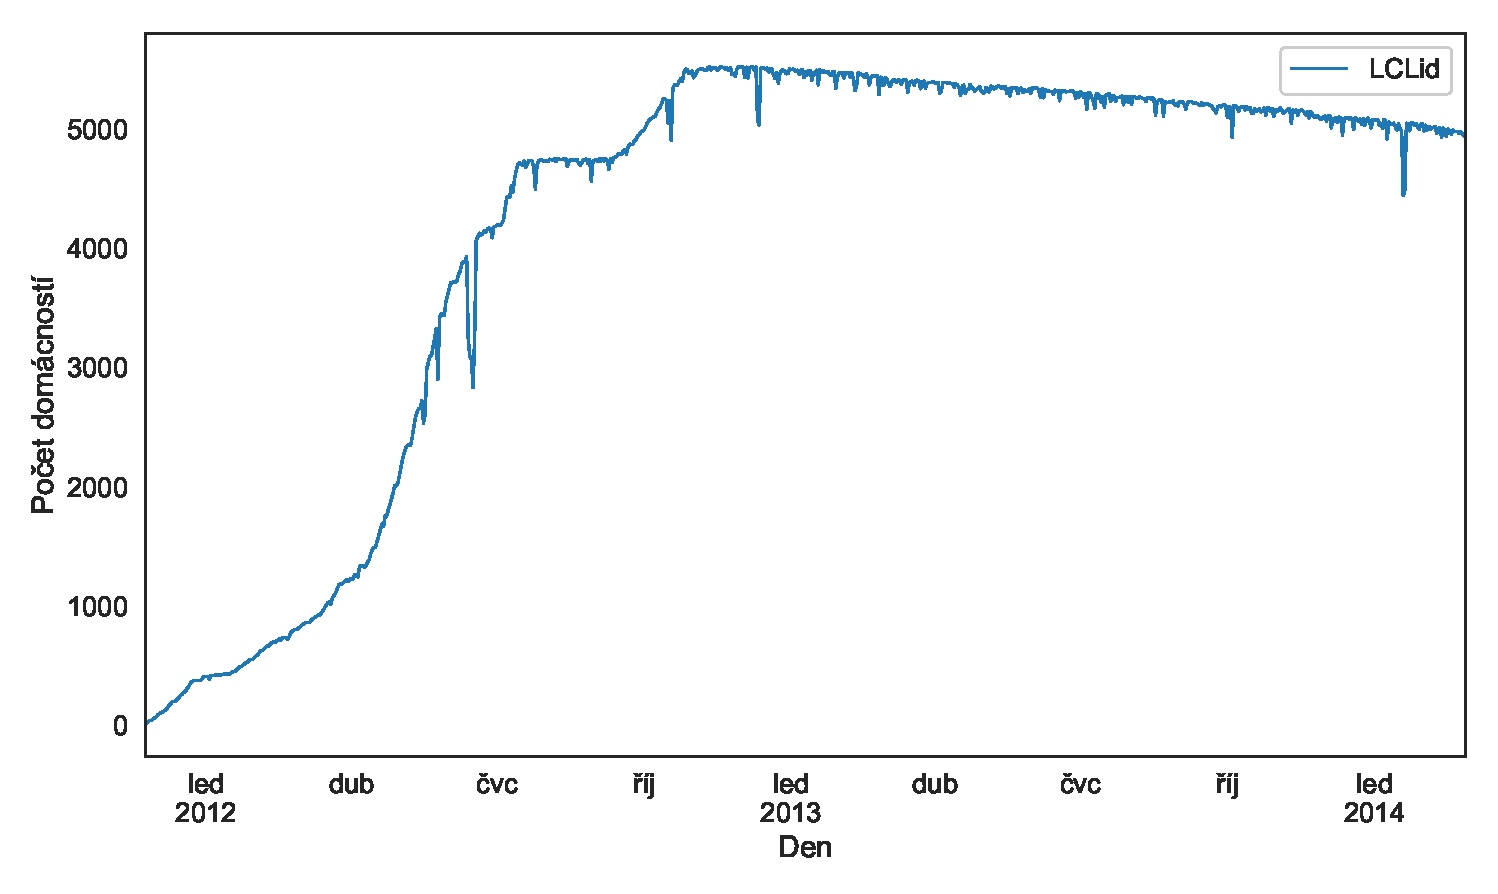
\includegraphics[width=0.7\textwidth]{pv_eda_01_households_over_time.eps}}%
	\caption{Graf s počtem zapojených domácností v čase }
	\label{fig:domacnosti-v-case}
\end{figure}

Po seskupení dnů v roce s identifikátorem domácnosti a zobrazení tohoto rozdělení na krabicovém grafu vypadají výsledky následovně:

\begin{figure}[htbp]
	\centering
	\makebox[\textwidth][c]{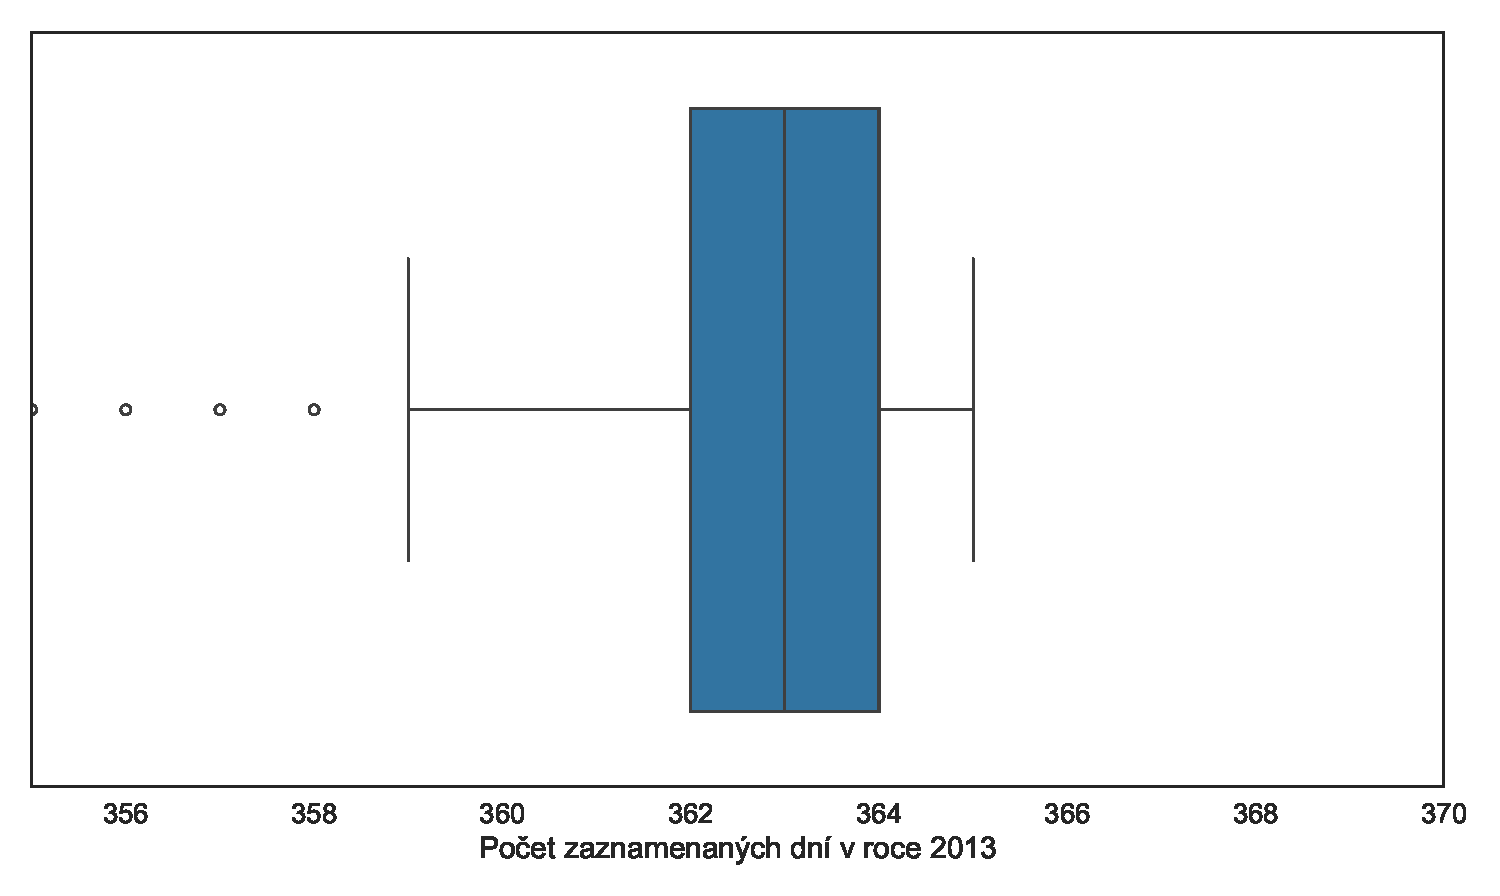
\includegraphics[width=0.7\textwidth]{number_of_records_distribution.eps}}%
	\caption{Graf rozdělení zaznamenaných dní pro domácnosti }
	\label{fig:domacnosti-v-case-pocet-dni}
\end{figure}


Z analýzy grafu výše vyplývá, že v rozsahu od 357 do 365 zaznamenaných dní dochází statisticky nejvýznamněji. S cílem zachovat kvalitu dat bylo rozhodnuto v datové sadě omezit výběr na domácnosti s alespoň 357 záznamy. Toto kritérium eliminuje 38 záznamů, což představuje pouze 0,68 \% z celkového objemu datové sady. Tímto opatřením lze zajistit relevantnější analýzu v rámci sledovaného rozsahu zaznamenaných dní.


\newpage

\subsection{Průměrné profily}
Jako první byly analyzovány hodinové průměry čtyř domácností. Byly vybrány tři domácnosti z datové sady z Londýna a jedna domácnost z Brna. Výsledky ukázaly, že průměrná spotřeba energie během dne výrazně kolísá mezi jednotlivými domácnostmi. To je způsobeno rozdílným chováním a užíváním spotřebičů obyvateli domácností.

Z grafu \ref{fig:hodina_pracovni} níže lze vidět, že u rezidence s identifikátorem 246 členové domácnosti začínají vstávat mezi 5-6. hodinou do práce. Tato aktivita se odráží v nárůstu spotřeby energie v těchto časných hodinách. Domu se vracejí kolem šesté, kde se pravděpodobně zapíná více spotřebičů (televize, mikrovlnná trouba, atd.). Podobný vzor lze nalézt i u rezidence 4431.

U zbytků rezidencí lze dle křivky předpokládat, že obyvatelé se vracejí domu kolem 15. hodiny a vstávají mezi 7-9. hodinou.
 
\begin{figure}[htbp]
	\centering
	\makebox[\textwidth][c]{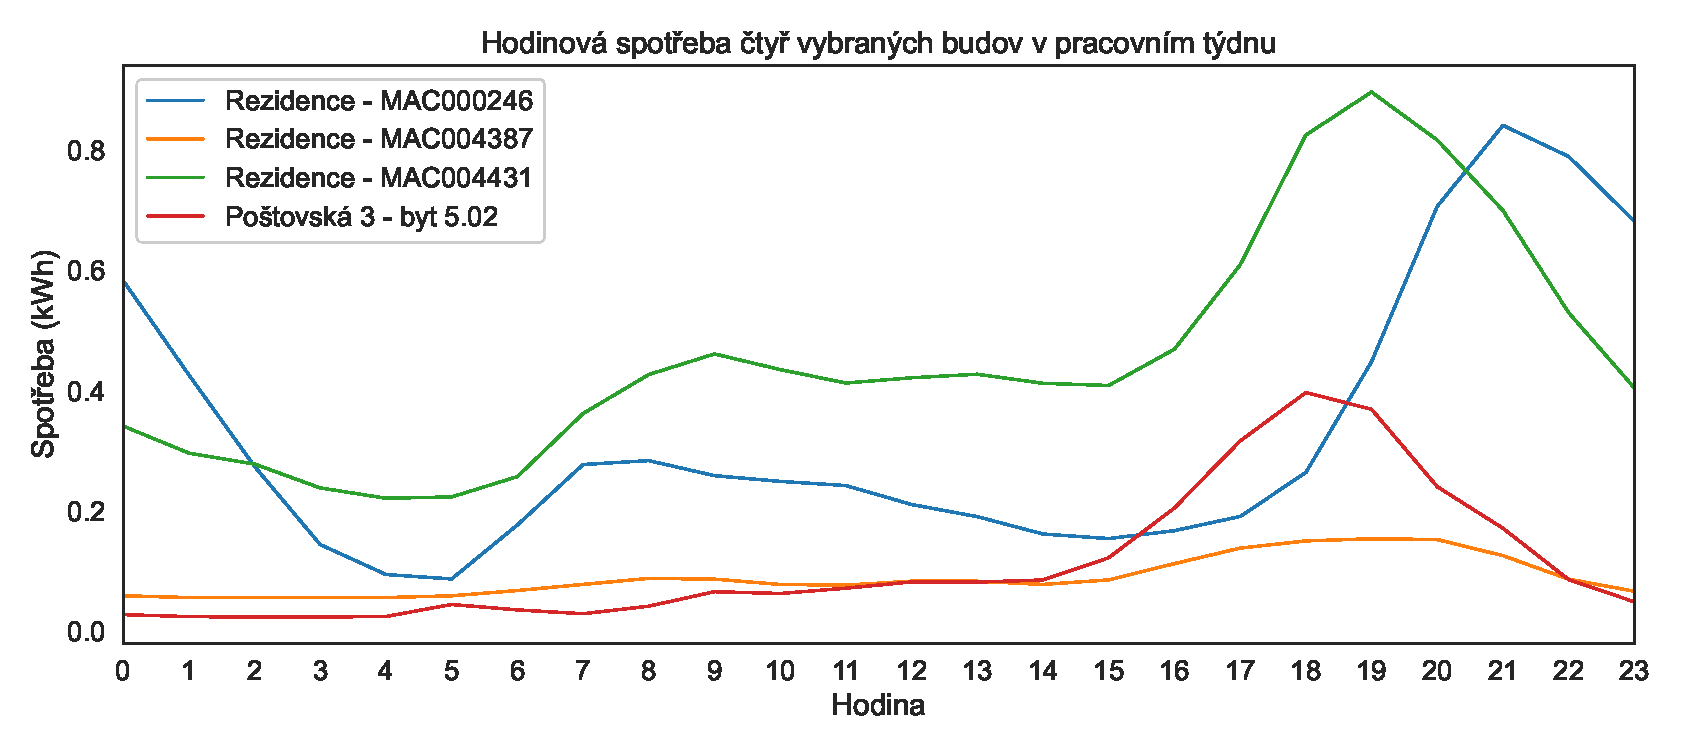
\includegraphics[width=1.0\textwidth]{pv_eda_01_week_avg_hour_group_weekend_0.eps}}%
	\caption{Hodinová spotřeba vybraných budov v pracovním týdnu}
	\label{fig:hodina_pracovni}
\end{figure}

Samotná informace o tom, jak vypadá hodinová spotřeba může být zajímavá v případě nějaké predikce chování uživatele, ovšem pro predikci spotřeby energie to příliš nepomůže. Proto ještě byl analyzován rozdíl mezi hodinovým průběhem pracovního týdne a víkendu.

Na grafu \ref{fig:hodina_vikend} níže lze zaznamenat signifikantní zvýšení spotřeby v průběhu dne o proti pracovním týdnu (hlavně na rezidenci 246). To se dá vysvětlit tím, že obyvatelé objektu pravděpodobně o víkendu nepracují a tráví raději čas doma.


Tento zjištěný rozdíl v hodinové spotřebě mezi pracovním týdnem a víkendem představuje jeden z klíčových příznaků \textit{is\_weekend} pro dále trénované modely. Kombinace  více příznaků totiž umožňuje vytvořit sofistikovanější model, který lépe predikuje a přizpůsobuje se dynamice spotřeby energie podle konkrétních situací, což může mít pozitivní dopad na efektivitu energetického řízení dané domácnosti.


\newpage

\begin{figure}[htbp]
	\centering
	\makebox[\textwidth][c]{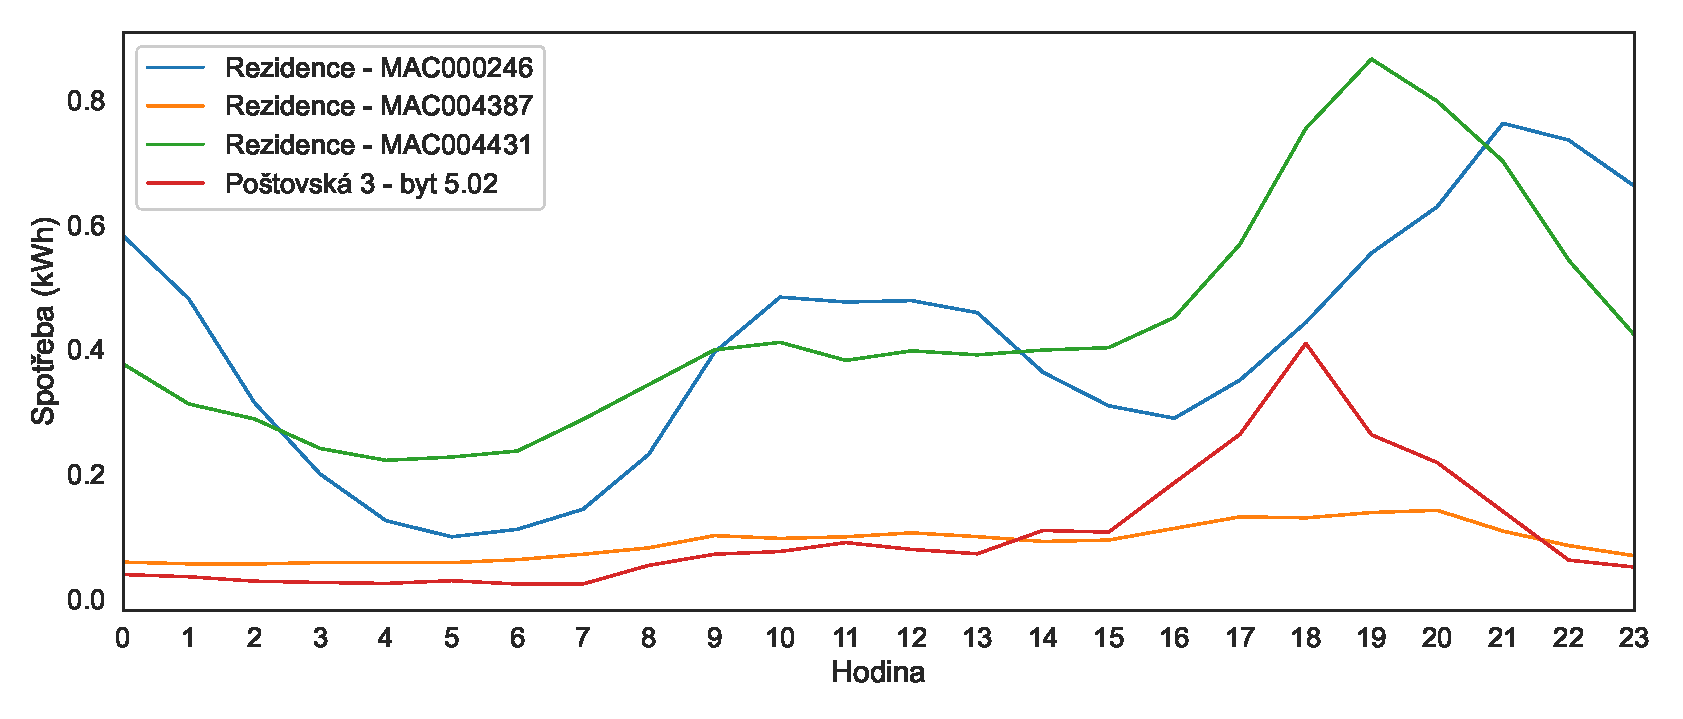
\includegraphics[width=1.0\textwidth]{pv_eda_01_week_avg_hour_group_weekend_1.eps}}%
	\caption{Hodinová spotřeba vybraných budov o víkendu}
	\label{fig:hodina_vikend}
\end{figure}

Pro úplnost byla provedena analýza hodinového profilů pro celou 10GB datovou sadu. Z grafu \ref{fig:hodina_all} je patrné, ve kterých hodinách obyvatelé domácnosti tráví čas doma. Tato analýza potvrzuje výsledky z hodinových průměrů vybraných čtyř domácností, které se od průměru příliš neliší.

\begin{figure}[htbp]
	\centering
	\makebox[\textwidth][c]{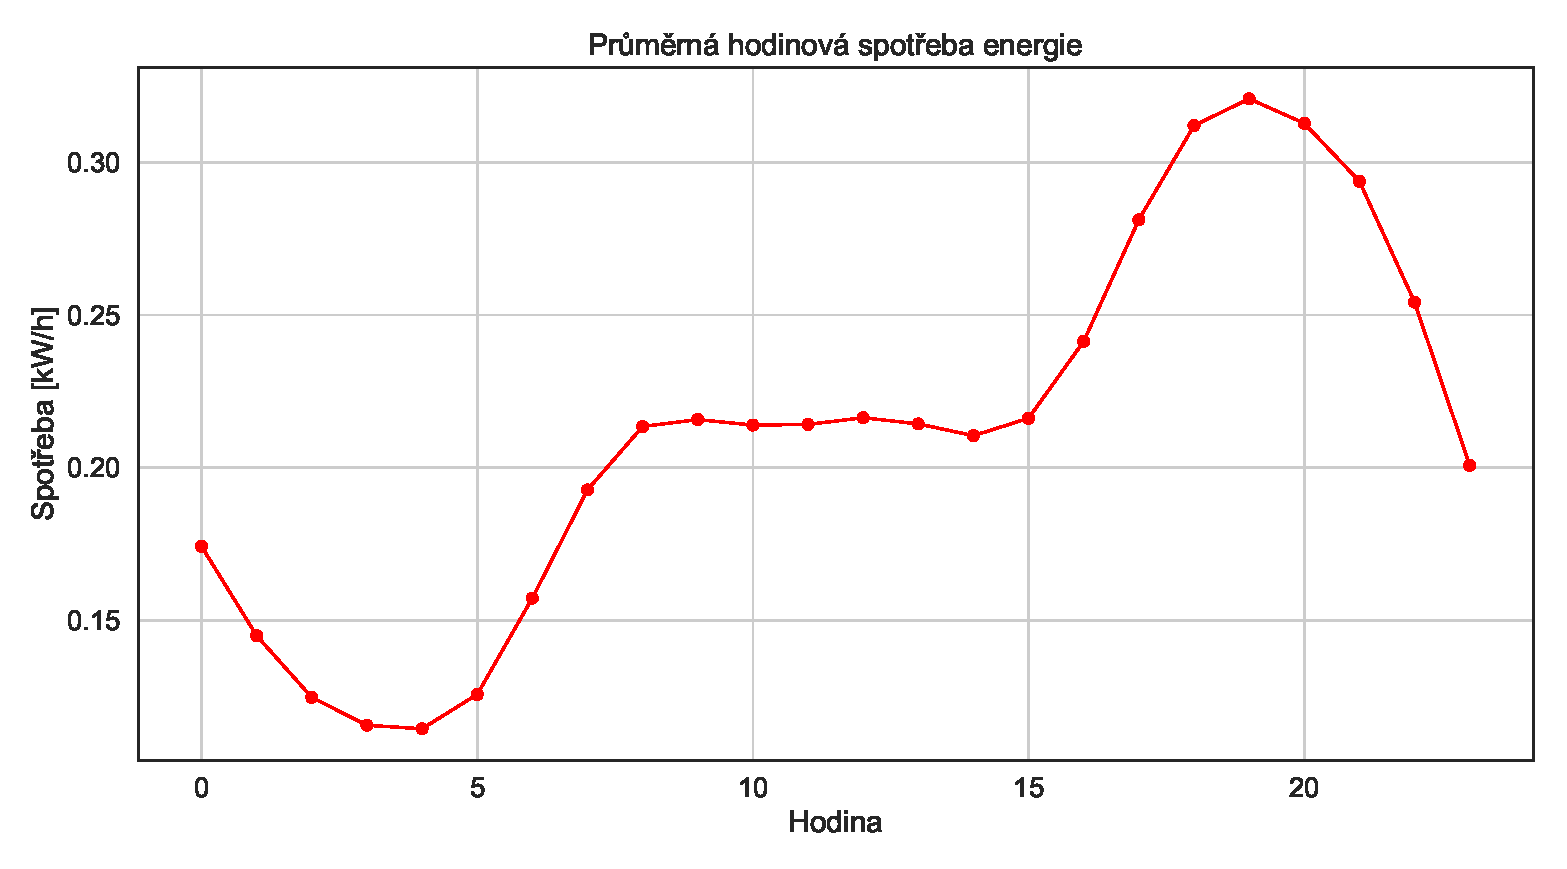
\includegraphics[width=0.8\textwidth]{pv_eda_01_week_avg_hourly_consumption_all.eps}}%
	\caption{Hodinová spotřeba všech domácností z datové sady}
	\label{fig:hodina_all}
\end{figure}

V rámci analýzy hodinových profilů bylo rovněž zkoumáno, zda roční období ovlivňuje spotřebu energie během jednotlivých dní. Výsledky odhalily souvislosti mezi sezónními změnami a spotřebou energie. Během zimních měsíců je zaznamenáván větší nárůst denní spotřeby energie, což může být způsobeno intenzivnějším využíváním vytápění v domácnostech.

Naopak během letních měsíců je zaznamenáván větší nárůst denní spotřeby energie, což může být způsobeno intenzivnějším využíváním klimatizačních systémů a dalších chladicích zařízení v domácnostech. \newpage

\begin{figure}[htbp]
	\centering
	\makebox[\textwidth][c]{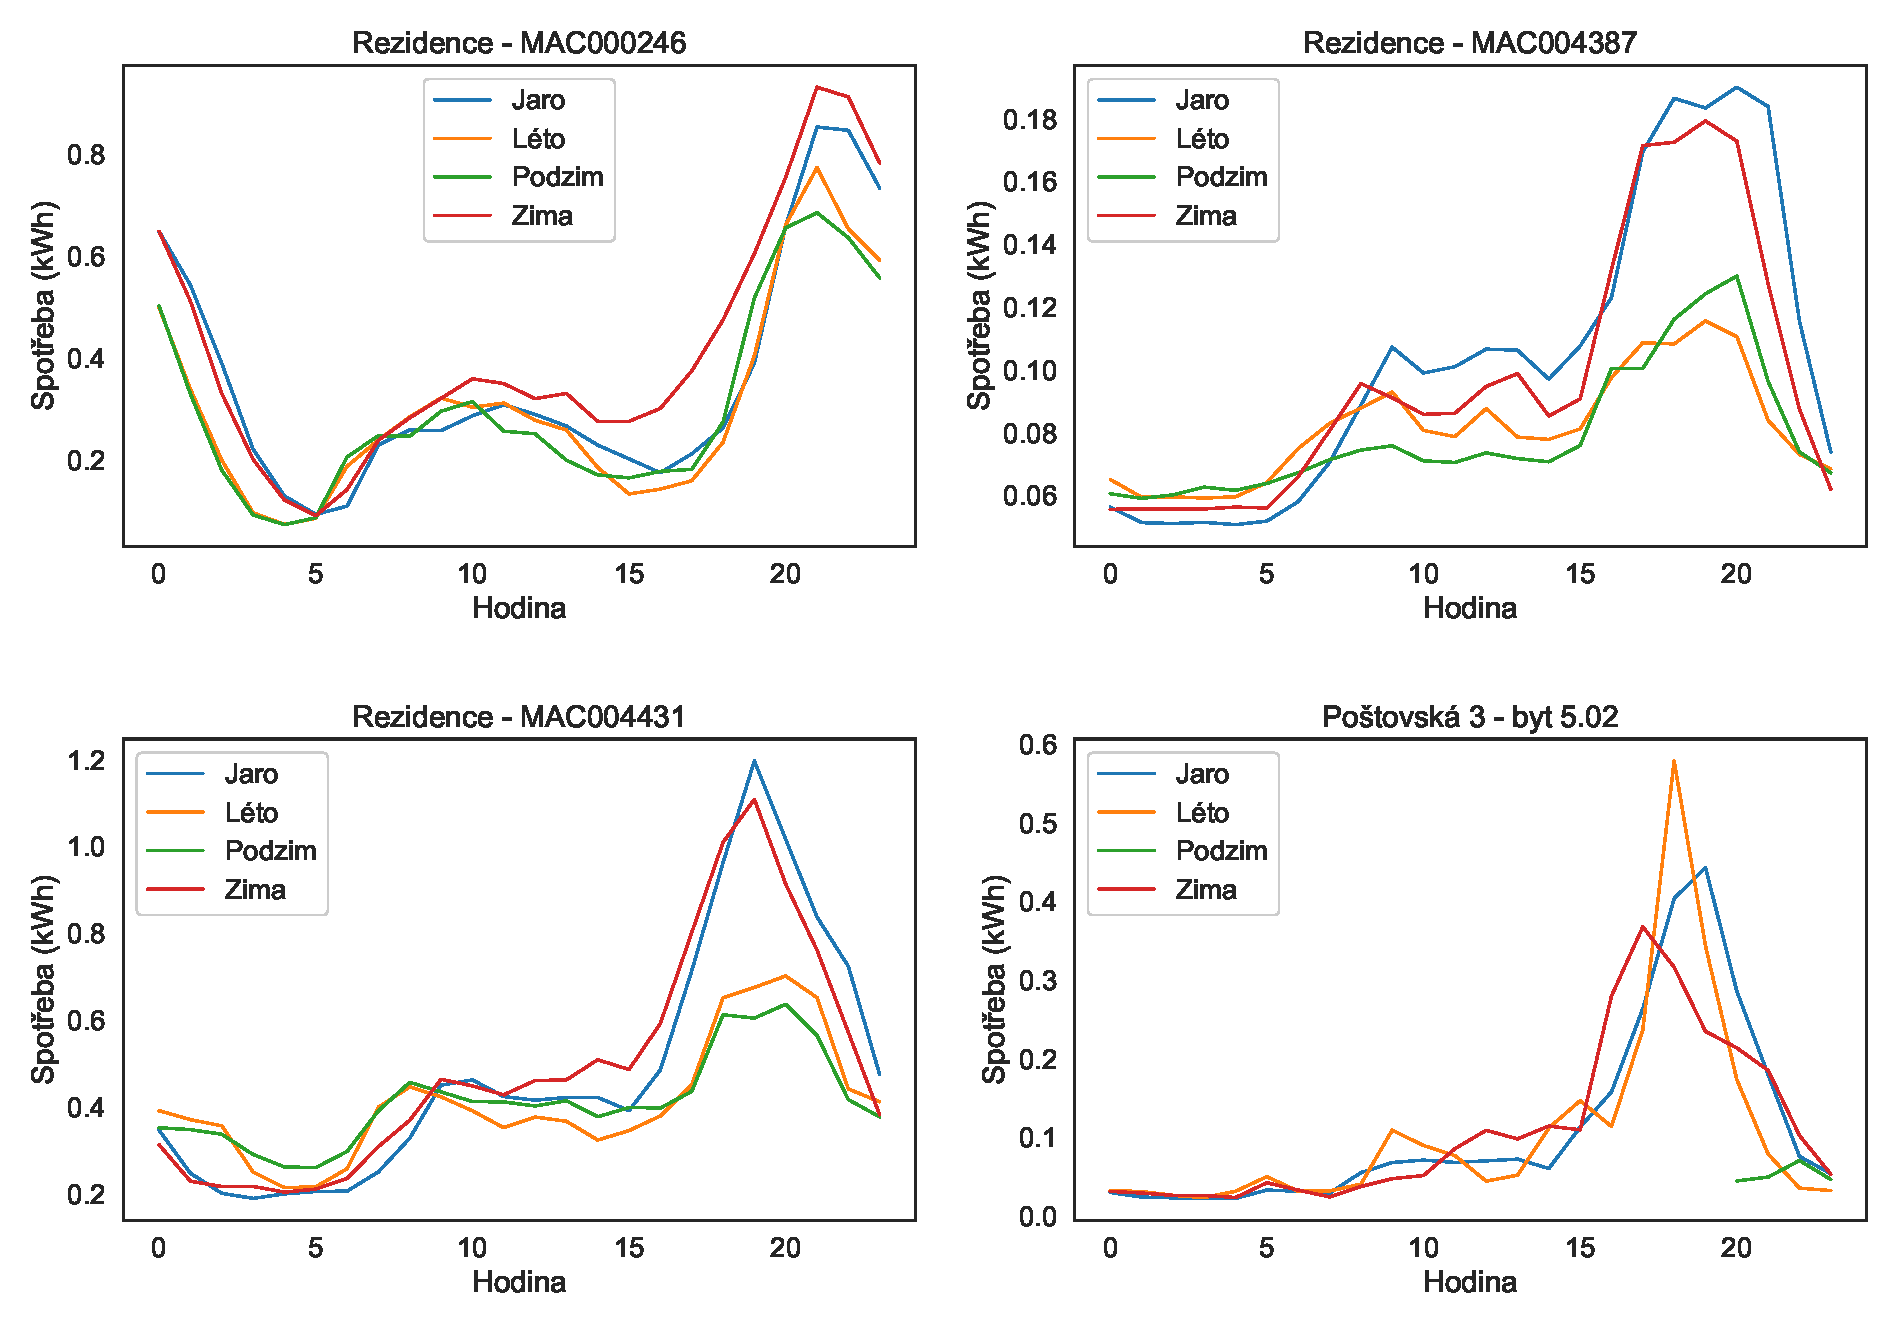
\includegraphics[width=0.8\textwidth]{hourly_energy_consumption_per_quarter.eps}}%
	\caption{Hodinová spotřeba vybraných domácností dle období}
	\label{fig:hodina_quarters}
\end{figure}

Na základě této provedené analýzy lze zařadit parametr \textit{quarter} jakožto indikátor ročního období mezi další příznaky, jenž bude model pro predikce využívat.

Další ze zkoumaných parametrů je závislost na dni v týdnu. Byl tedy vytvořen průměrný týdenní profil vybraných domácností. Tento profil by mohl obsahovat důležité informace pro lepší pochopení dynamiky spotřeby energie v průběhu týdne. 

\begin{figure}[htbp]
	\centering
	\makebox[\textwidth][c]{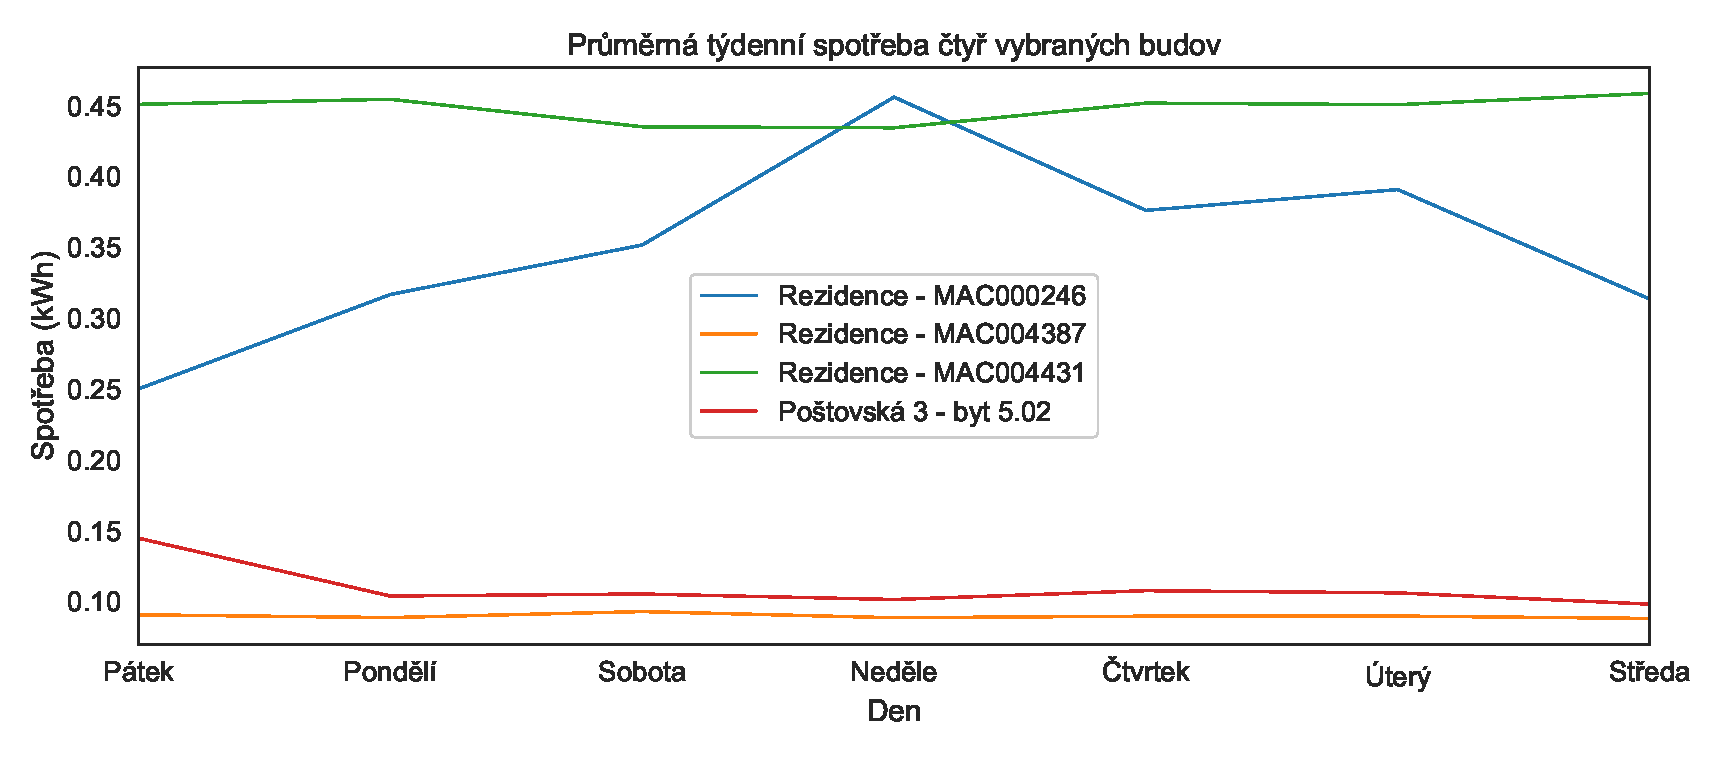
\includegraphics[width=0.8\textwidth]{pv_eda_01_week_avg_daily_consumption_group.eps}}%
	\caption{Denní průměrný profil vybraných domácností v týdnu}
	\label{fig:tyden_avg_group}
\end{figure}

Z grafu \ref{fig:tyden_avg_group} je na první pohled vidět, že někteří obyvatelé rádi tráví čas o víkendech doma (obyvatelé domácnosti 246) a jiní raději tráví čas mimo domov (obyvatelé domácnosti 4431), což vysvětluje snížení či zvýšení spotřeby o víkendu. To znamená, že je to jeden z relevantních indikátoru pro odhadování spotřeby energie. Z tohoto důvodu bude i příznak \textit{week\_day} použit v následujících modelech pro predikci.

Poslední příznak z časově závislých parametrů, jenž byl zkoumán je závislost spotřeby na dni v roce. Zde se předpokládá sezonní trend, obdobný jako příznak \textit{quarter}, který vykazoval v zimních a letních měsících variaci oproti zbytku. 

Pro každou domácnost v analýze byl tedy proveden denní průměr spotřebované energie přes celý rok 2013. 

\begin{figure}[htbp]
	\centering
	\makebox[\textwidth][c]{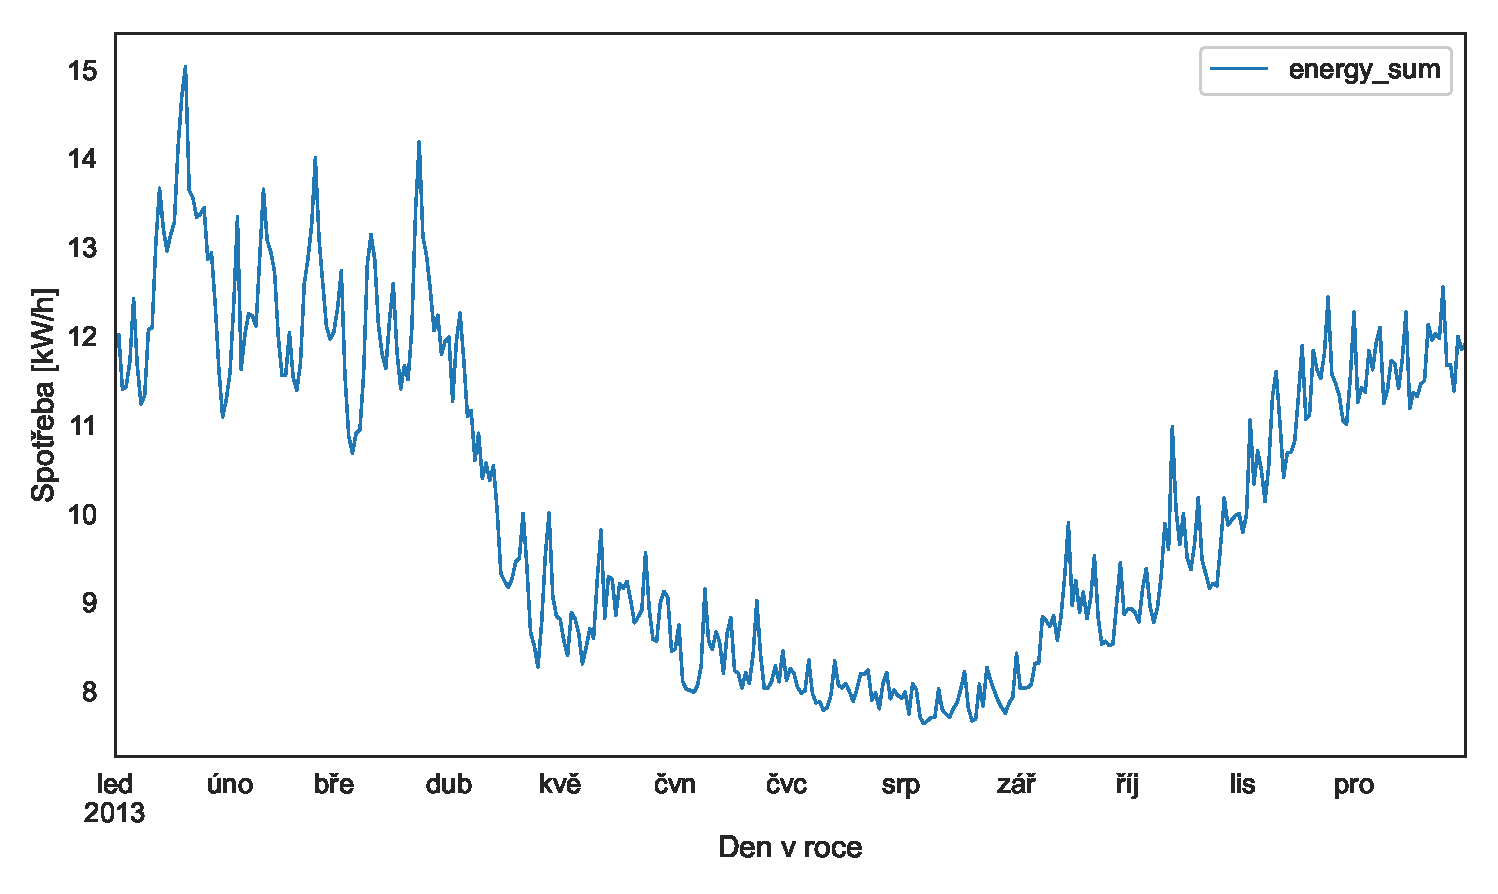
\includegraphics[width=0.8\textwidth]{pv_eda_01_daily_consumption_all.eps}}%
	\caption{Denní průměrný profil vybraných domácností v roce}
	\label{fig:year_avg_all}
\end{figure}

Z grafu \ref{fig:year_avg_all} se potvrzuje, že zde existuje závislost mezi spotřebovanou energií a dnem v roce. Sezonní efekt lze vidět v měsících, kde je zpravidla větší zima, což by indikovalo, že mnoho lidí využívá elektrický zdroj pro vytápění své domácnosti. Parametr \textit{day} bude zařazen do seznamu příznaků v modelech.

\subsection{Závislost počasí}
V předchozí kapitole byla odkryta závislost na ročním období, proto je vhodné prozkoumat závislosti spotřeby na parametrech z datové sady o počasí popsanou v tabulce \ref{weather_dataset}.

K tomu, aby bylo možné provést takovou analýzu, je nutné spojit obě datové sady do jedné. Taktéž musí být vzato v úvahu, že údaje o spotřebě jsou měřeny v půlhodinových intervalech, zatímco meteorologická data jsou dostupná v hodinových intervalech. S cílem zabránit ztrátě informací, bude i počasí interpolováno na půlhodinové intervaly.

Pro tento účel byla využita lineární interpolace, přičemž pokud hodnota bude v datové sadě chybět, doplní poslední změřenou hodnotu teploty.

Analýza byla provedena na celé datové sadě. Byla spočítána průměrná denní teplota a průměrná denní spotřeba energie. Graf zobrazující tento vztah vypadá následovně:

\begin{figure}[htbp]
	\centering
	\makebox[\textwidth][c]{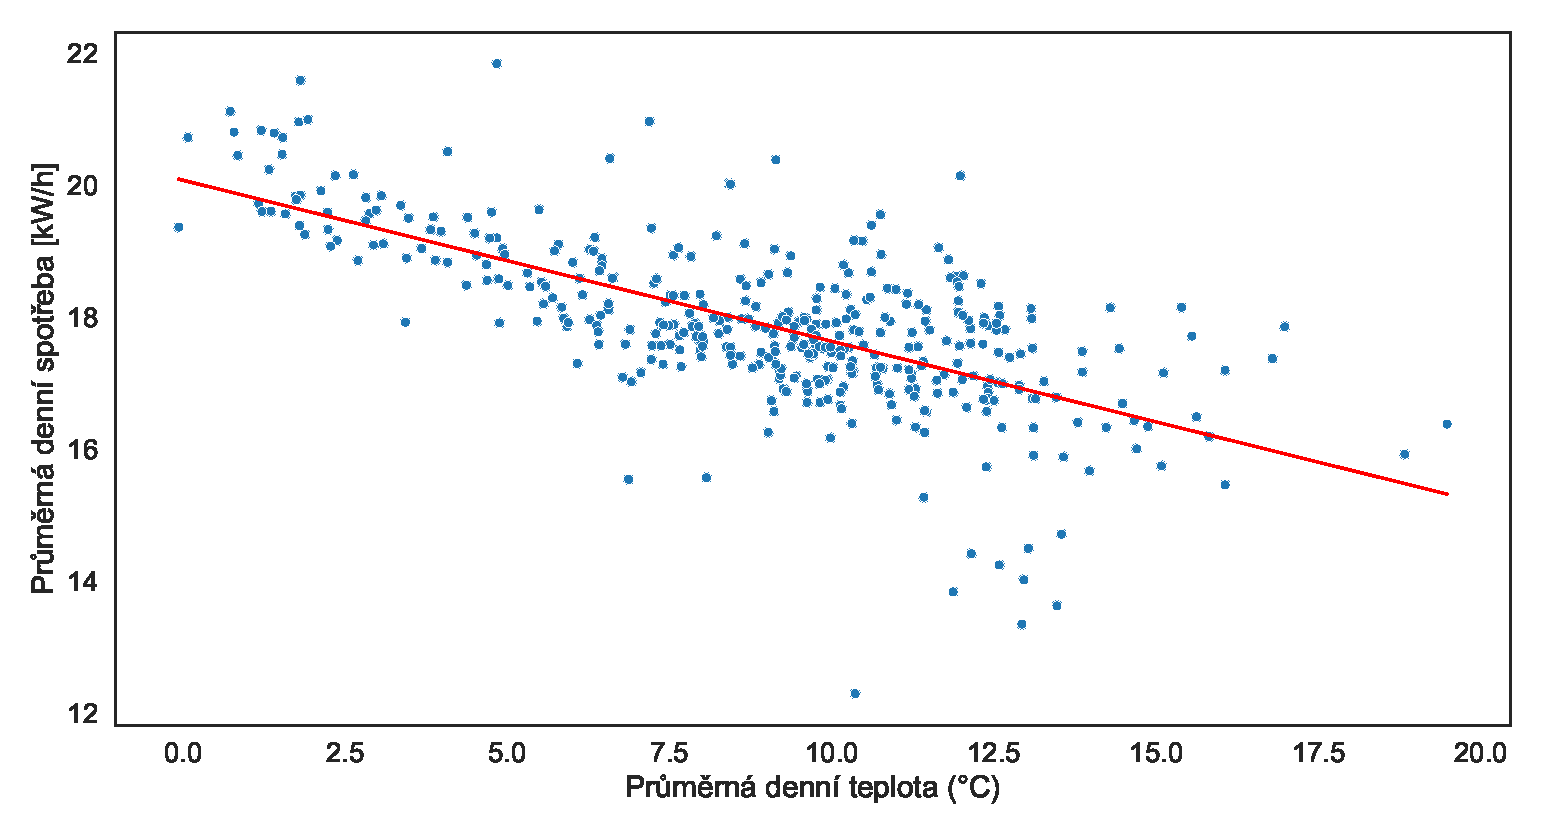
\includegraphics[width=0.8\textwidth]{pv_eda_02_weather_over_consumption.eps}}%
	\caption{Vztah mezi průměrnou denní spotřebou a průměrnou denní teplotou}
	\label{fig:year_avg_all}
\end{figure}

Z grafu lze na první pohled vidět, že zde je trend a to klesající, jinými slovy, se zvyšující se teplotou klesá spotřebovaná energie. To může být způsobeno tím, že objekty v datové sadě využívají elektrického tepelného vytápění. Jelikož z grafu je patrný trend, byl příznak teploty zařazen pro použití ve finálních modelech.

Datová sada s počasím má ovšem mnohem více parametrů, které by mohly být důležité pro predikci. Pro identifikování parametrů, které by měly být zařazeny do finálního modelu, bylo využito výpočtu pro změření velikosti lineární závislosti mezi jednotlivými parametry. Bylo využito Pearsonova korelačního koeficientu. Korelační koeficient se počítá dle následujícího vzorce: 

\begin{equation}
	r =
	\frac{ \sum_{i=1}^{n}(x_i-\bar{x})(y_i-\bar{y}) }{%
		\sqrt{\sum_{i=1}^{n}(x_i-\bar{x})^2}\sqrt{\sum_{i=1}^{n}(y_i-\bar{y})^2}}
\end{equation}

kde ve jmenovateli jsou násobeny směrodatné odchylky obou proměnných a v čitateli se počítá kovariance. Jelikož se zde dělí směrodatnou odchylkou, výsledný koeficient $r$ vyjde jako normované bezrozměrné číslo v rozsahu -1 až 1.

Interpretace hodnoty $r$ spočívá v tom, že čím blíže je hodnota korelačního koeficientu k 1 nebo -1, tím silnější je lineární vztah mezi dvěma proměnnými. Hodnota $r$ blízká 0 naznačuje, že mezi proměnnými není lineární vztah.

Kromě toho, že tento koeficient umožňuje náhled na proměnné, které by mohly být užitečné, tak umožňuje i redukci dimenze vstupních dat pro predikční model. Pomocí korelační matice je totiž možné zobrazit všechny korelační koeficienty pohromadě a rozhodnout, které proměnné v datové sadě jsou redundantní na základě znalosti hodnoty $r$.

V této práci bylo využito implementace korelačního koeficientu v knihovně \textit{pandas}. Sloupce, které jsou textovém tvaru (např. $precipType$), byli převedeny na číselné hodnoty 0 až $n$, kde $n$ je počet unikátních položek. Korelační matice zobrazující vztah mezi spotřebou energie a počasím vypadá takto:

\begin{figure}[htbp]
	\centering
	\makebox[\textwidth][c]{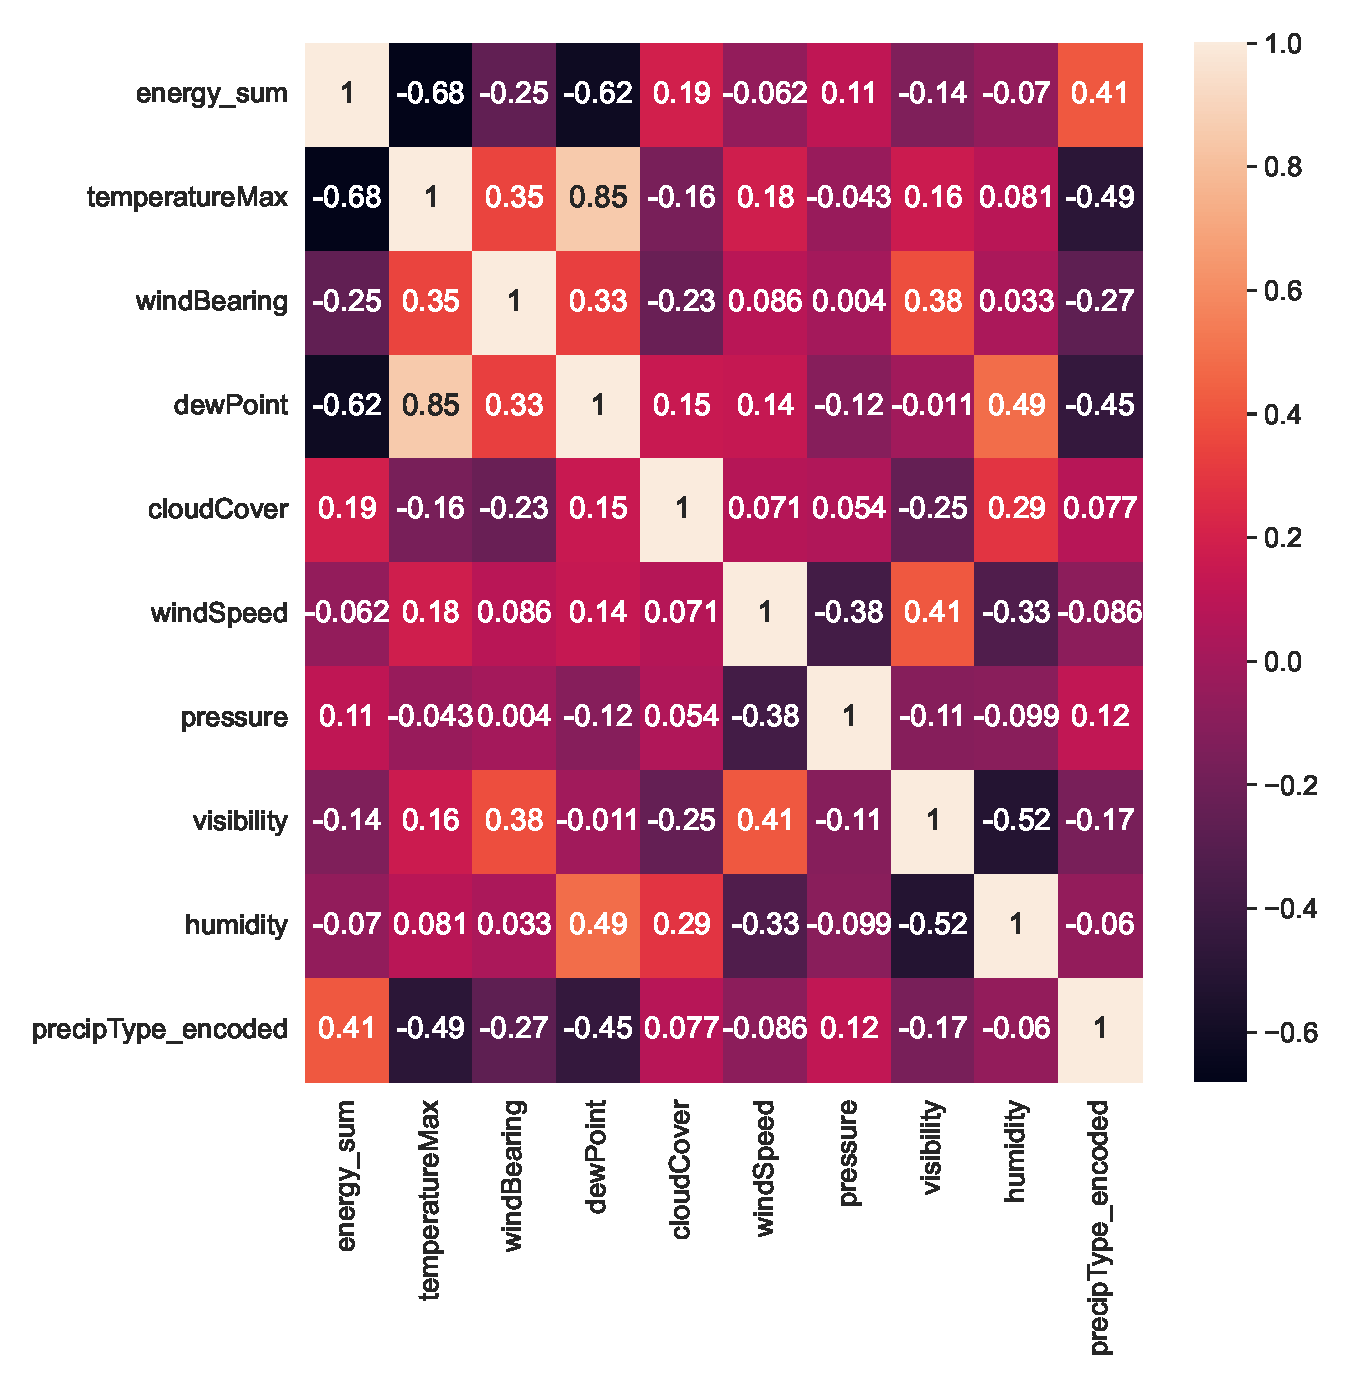
\includegraphics[width=0.6\textwidth]{pv_eda_02_heat_weather.eps}}%
	\caption{Ilustrační korelační matice zobrazující vztah mezi spotřebou a počasím}
	\label{fig:year_avg_all}
\end{figure}

Z matice vyplývá, že \textit{vlhkost} a \textit{rychlost větru} nemají téměř žádnou závislost na spotřebě energie. Naopak proměnná \textit{dewPoint}, neboli rosný bod, vykazovala výraznější vztah ke spotřebě energie, avšak její korelace s teplotou byla příliš vysoká. Proto byla tato proměnná vynechaná z finálního seznamu proměnných, aby se předešlo redundanci a zjednodušila se interpretace výsledků.

Na základě této analýzy byly zvoleny parametry \textit{temperature}, \textit{pressure}, \textit{windBearing}, \textit{precipType} a \textit{visibility}.

Dále byl proveden výpočet korelační matice i pro proměnné, které byly zkoumány v předchozích fázích analýzy (TODO: velká matice do přílohy). Ná základě hodnot koeficientu $r$ vyšlo, že parametr \textit{quarter} je nadbytečný, jelikož silně koreluje s parametrem \textit{month} ($r=0.98$) a silně také koreluje s parametrem \textit{day} ($r=0.97$). Proto byl tento parametr ze vstupních dat pro predikční modely odstraněn. Další analýza dat, jako je například autokorelace, bude provedena v následujících kapitolách zabývajících se samotnou implementací modelů.


\newpage

\section{Implementace jednotlivých modelů}

Na základě předchozí explorační analýzy byly zvoleny následující společné proměnné pro všechny modely. 

\begin{table}[!ht]
	\centering
	\caption{Společné parametry pro všechny predikční modely}
	\label{weather_dataset}
	\begin{tabularx}{\linewidth}{lX}
		\hline
		\textbf{Sloupec} & \textbf{Popis} \\ \hline
		visibility & Maximální viditelnost \\ 
		windBearing & Směr, ze kterého fouká vítr \\ 
		temperature & Skutečná teplota ve stupních Celsia \\ 
		pressure & Aktuální atmosférický tlak měřený v hektopascálech. \\ 
		precipType & Typ srážky (sníh nebo déšť) \\
		hour & Hodina, kdy byl vytvořen záznam \\
		minute & Minuta, kdy byl vytvořen záznam \\
		month & Měsíc, kdy byl vytvořen záznam \\
		year & Rok, kdy byl vytvořen záznam \\
		energy(kWh/hh) & Spotřebovaná energie v kWh \\
		\hline
	\end{tabularx}
\end{table}

Tyto proměnné slouží pouze jako základ pro veškeré modely. Některé z modelů využívají navíc ještě uměle vytvořené proměnné (např. zpožděné proměnné u xgboost modelu), pro zpřesnění predikcí.

Výsledné modely jsou serializované v souboru s příponami \textit{.h5} pro LSTM a \textit{.pkl} pro XGBoost. Tato serializace umožňuje uchování modelů pro opakované a přenosné použití bez nutnosti opakovaného trénování.

\subsection{XGBoost}
V kapitole \ref{xgboost_research} v rešeršní části práce bylo zmíněno, že xgboost využívá \textit{ensemble} metody, které kombinují slabší modely, jenž jsou na sobě trénovány nezávisle. Z toho plyne, že se zde nevychází z časového uspořádání, což je pro přesnou predikci časové řady klíčové.

Proto bylo nejdříve nezbytné najít řešení pro včlenění časového uspořádání do modelu XGBoost, který standardně nezohledňuje informace o času. Jednou z metod, jak toho dosáhnout, je vytvoření umělých zpožděných proměnných (lag features). Tyto proměnné obsahují informaci o minulých hodnotách cílové proměnné nebo jiných relevantních faktorech v daných časových oknech.

Pro tento účel byl proveden experiment, ve kterém byly postupně vybírány vhodné zpožděné proměnné. Tyto proměnné byly vytvořeny na základě explorační analýzy datové sady. Do modelu byly zahrnuty proměnné, které obsahují informaci o minulých hodnotách vybraných proměnných v různých časových oknech, což umožňuje modelu lépe zachytit trendy časové řady a vzory v datech. 

Výsledná tabulka se zpožděnými proměnnými vypadá následovně: 

\begin{table}[!ht]
	\centering
	\caption{Zpožděné proměnné pro XGBoost model}
	
	\begin{tabularx}{\linewidth}{lX}
		\hline
		\textbf{Parametr} & \textbf{Popis} \\ \hline
		energyMean6 & průměrná hodnota spotřeby energie v posledních šesti hodinách \\
		energyMean12 & průměrná hodnota spotřeby energie v posledních dvanácti hodinách \\
		energyMean24 & průměrná hodnota spotřeby energie za poslední den \\
		energyMax6 & maximální hodnota spotřeba energie za posledních 6 hodin\\
		energyMin6 & minimální hodnota spotřeby energie za posledních 6 hodin\\
	\end{tabularx}
\end{table}


Jako další umělá proměnná byla zvolena první a druhá diference. Tyto diference byly zahrnuty z důvodu jejich schopnosti zachytit změny a trendy v datech o spotřebě energie, což je klíčové pro přesnou predikci budoucích hodnot spotřeby. První diference reprezentuje okamžité změny v hodnotách dat, které si dokážou poradit s náhlými výkyvy spotřeby energie. 

Trénovací a testovací data byla rozdělena na 70 \% trénovacích a zbylých 30 \% na testování. Kromě toho existuje měsíc dat, jenž je kompletně mimo datovou sadu, na které probíhala validace (out-of-sample data). 


Volba hyper-parametrů pro výsledný model probíhala experimentální metodou. Nakonec došlo k volbě následujících parametrů:

\begin{table}[!ht]
	\centering
	\caption{Parametry finálního modelu}
	
	\begin{tabularx}{\linewidth}{lX}
		\hline
		\textbf{Parametr} & \textbf{Hodnota} \\ \hline
		booster & gbtree \\
	    objective & reg:squarederror \\
		eval\_metric & logloss \\
		eta & 0.01 \\
		learning\_rate & 0.02 \\
		max\_depth & 6\\
		base\_score  & 0.5\\
		n\_estimators  & 1000\\
	\end{tabularx}
\end{table}

Gradientní boostované rozhodovací stromy lze snadno analyzovat a interpretovat díky jejich \textit{ensemble} architektuře. Proto je možné jednoduše zjistit jak moc důležité jsou jednotlivé parametry pro rozhodování natrénovaného modelu. Pro výpočet skóre důležitosti příznaků byla využita diagnostická funkce \textit{plot\_importance}, kterou poskytuje knihovna XGBoost v Pythonu. Toto skóre udává, jak moc každá proměnná přispívá k rozhodování modelu a napomáhá k vyřazení nepotřebných příznaků za účelem optimalizace a zvýšení přesnosti. 
 
 \begin{figure}[htbp]
 	\centering
 	\makebox[\textwidth][c]{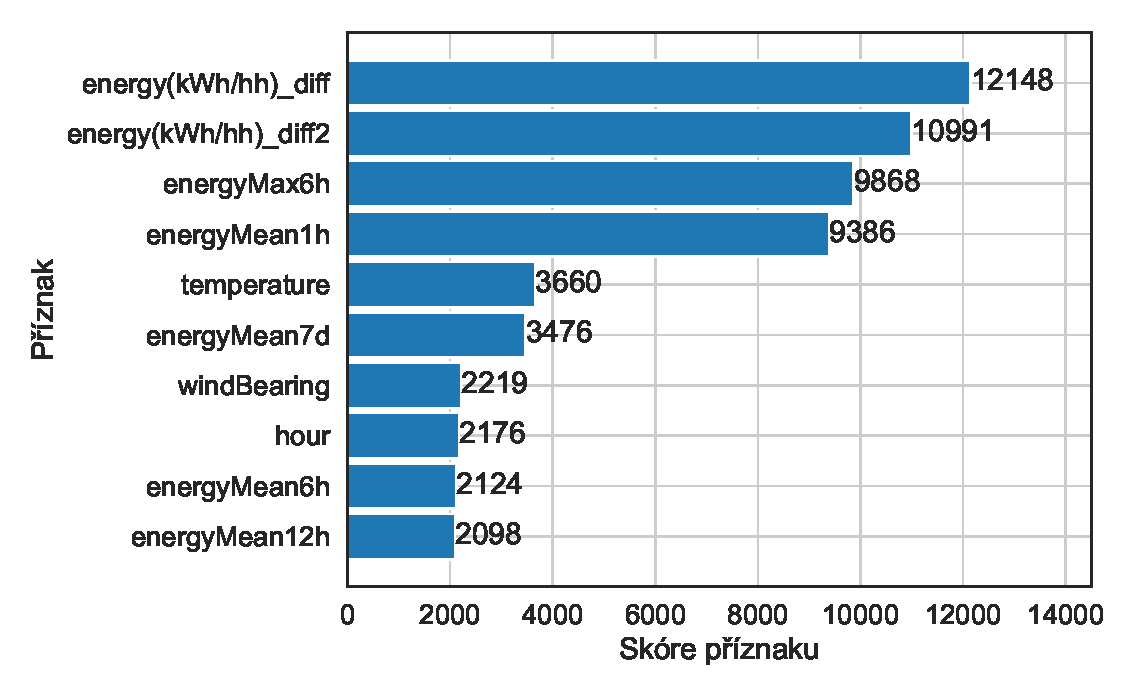
\includegraphics[width=0.6\textwidth]{xgboost_f_score.eps}}%
 	\caption{Skóre důležitosti pro 10 nejlepších příznaků}
 	\label{fig:xgboost_f_score}
 \end{figure}
 
Graf \ref{fig:xgboost_f_score} zobrazuje 10 příznaků s nejvyšším dosaženým skóre. Touto analýzo bylo zjištěno, že proměnné obsahující diferenci, teplotu a hodinu (či její průměry) jsou nejdůležitějšími příznaky při rozhodování modelu. Na základě tohoto grafu byly vyřazeny příznaky jako \textit{is\_weeeknd} či \textit{pressure}.

Pro objektivní zhodnocení, jak moc dobře se model přizpůsobuje validačním datům a zdali nedochází k přeučení a tím k nedostatečné generelizaci modelu, byl použit ukazatel ztráty. Tento ukazatel měří, jak úspěšně model minimalizuje rozdíl mezi předpovídanými a skutečnými hodnotami na trénovacích a validačních datech.


\begin{figure}[htbp]
	\centering
	\makebox[\textwidth][c]{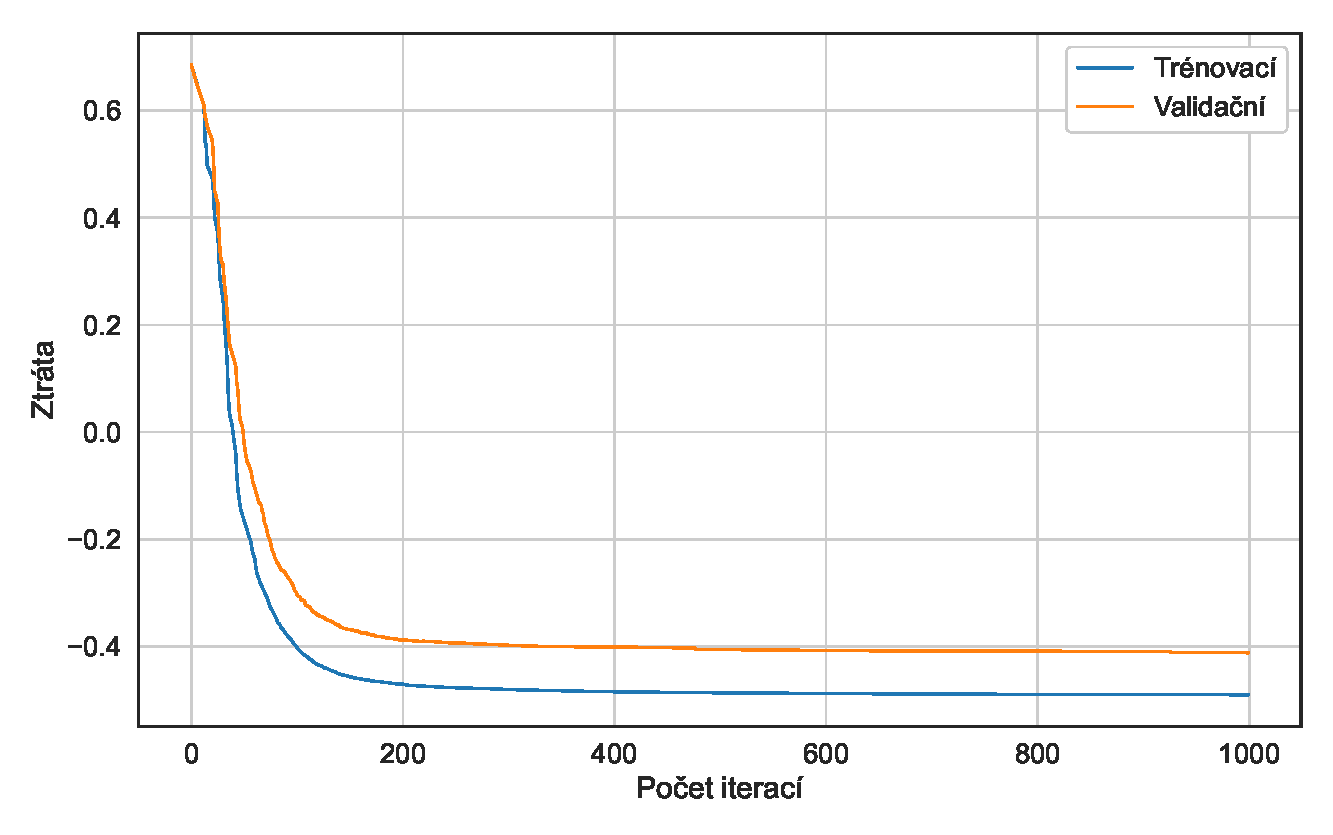
\includegraphics[width=0.6\textwidth]{xgboost_learning_curve.eps}}%
	\caption{Křivka učení finálního XGBoost modelu}
	\label{fig:xgboost_learning_curve}
\end{figure}

Na grafu \ref{fig:xgboost_learning_curve} výše lze vidět, že validační ztráta se ustálila na jedné úrovni a dále nemá tendenci vzrůstat. Zároveň je trénovací a  validační ztráta blízko k sobě. To naznačuje, že se model dobře přizpůsobuje datové sadě a nemělo by zde dojit k přeučení.

Finální natrénovaný model na validační množině dosahuje hodnot průměrné absolutní odchylky \textbf{5.36 \%}. Na grafu \ref{fig:xgboost_predictions} níže je vidět ukázka predikce pro jeden a půl dne dopředu.

\begin{figure}[htbp]
	\centering
	\makebox[\textwidth][c]{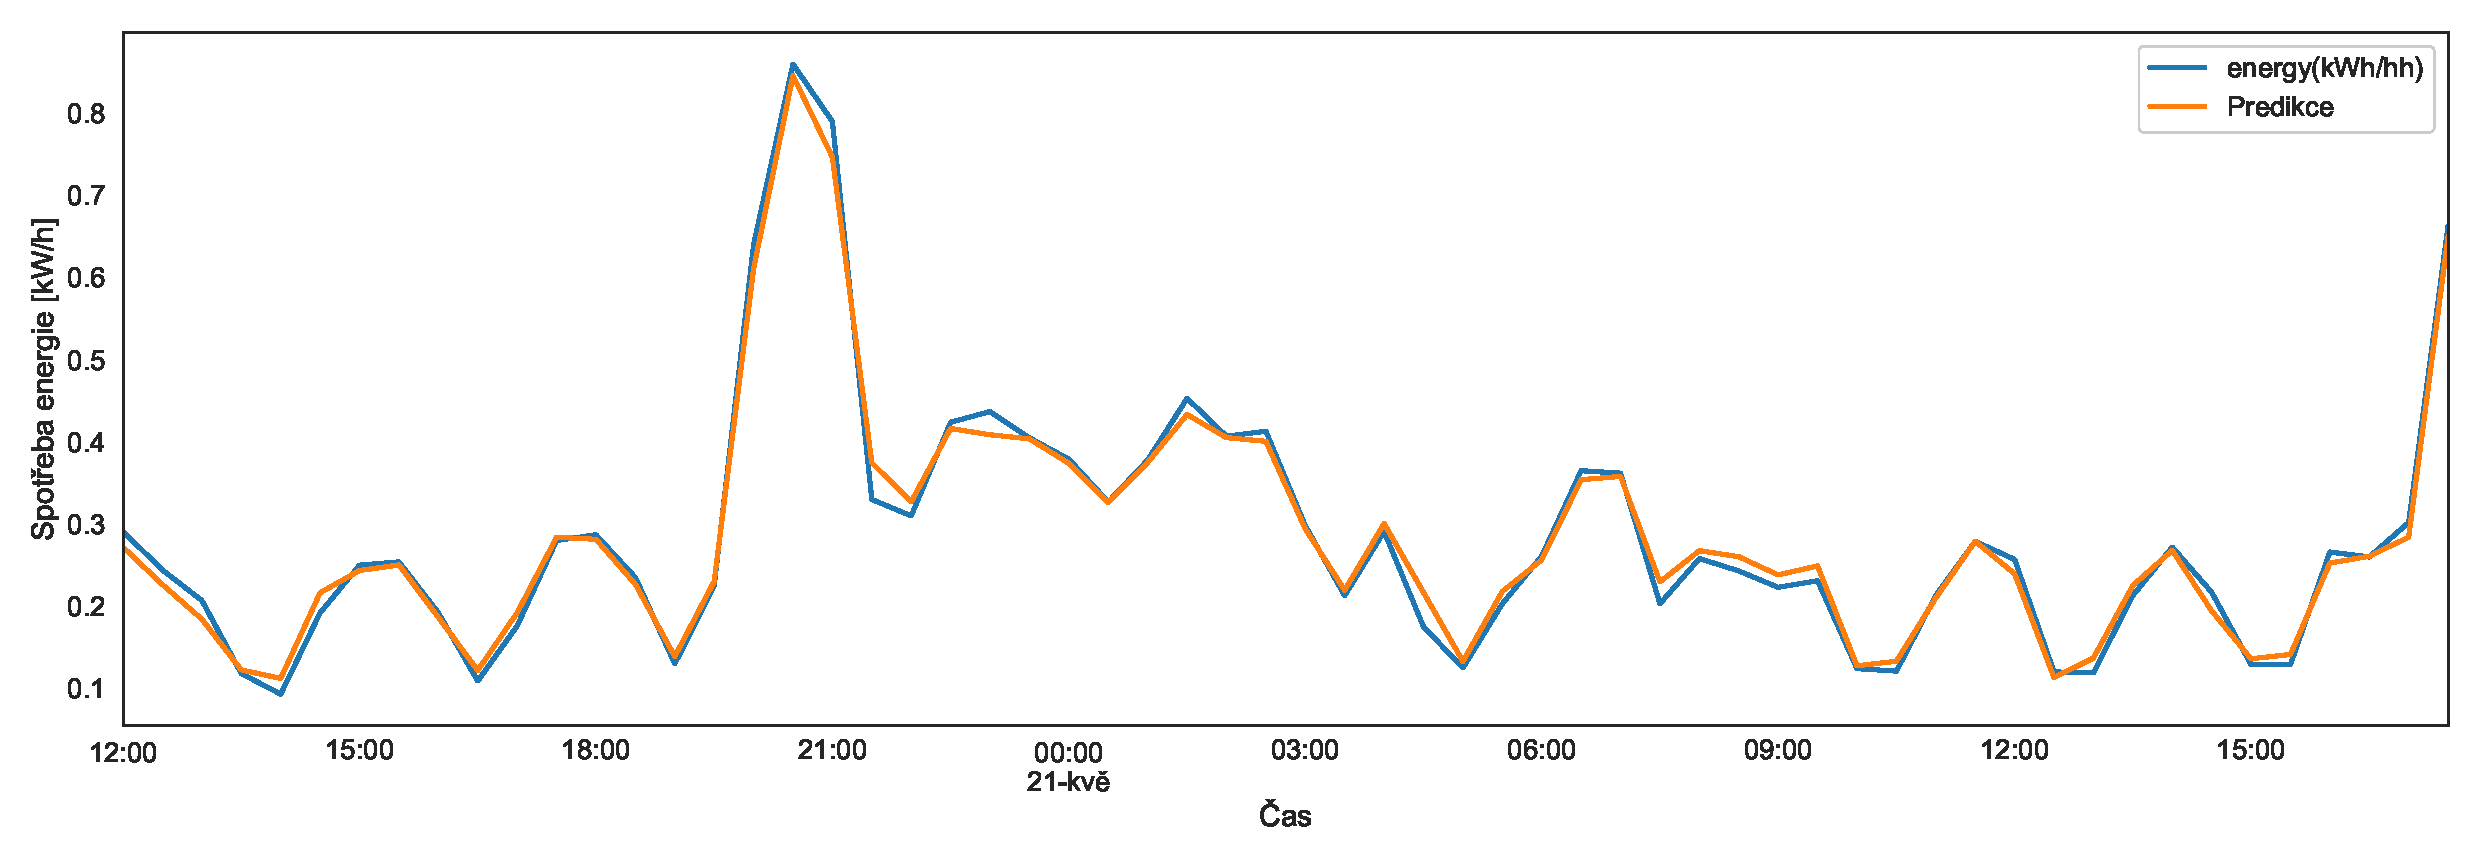
\includegraphics[width=0.9\textwidth]{xgboost_predictions.eps}}%
	\caption{Výřez predikce na validační datové sadě}
	\label{fig:xgboost_predictions}
\end{figure}


\subsection{ARIMA}
Ukázat jak byla udělána autokorelace a výběr jednotlivých parametrů....


\newpage
\subsection{LSTM}
Pro finální verzi LSTM modelu byly zvoleny následující parametry. Pro rychlejší a stabilnější konvergenci modelu během trénování byl zvolen optimalizační algoritmus jménem Adam. Jako chybová funkce (loss function) $L(x,y|w)$ byla použita MSE. 
Optimální velikost dávky (batch size) byla nastavena na hodnotu 128. 

\begin{table}[!ht]
	\centering
	\caption{Výsledná architektura LSTM sítě}
	
	\begin{tabularx}{\linewidth}{llXXX}
		\hline
		\textbf{Vrstva} & \textbf{Neurony} & \textbf{Výstupní rozměr} & \textbf{Počet parametrů} & \textbf{Ostatní nastavení} \\ \hline
		LSTM & 50 & (None, 1, 50) & 19 800 & returnSequences=True \\
		Dropout & - & (None, 1, 50) & 0 & - \\
		LSTM  & 75 & (None, 1, 75) & 37 800 & returnSequences=True \\
		Dropout & - & (None, 1, 75) & 0 & - \\
		LSTM   & 50 & (None, 50) & 25 200 & returnSequences=False \\
		Dropout & - & (None, 50) & 0 & - \\
		Dense & - & (None, 1) & 51 & units=1 \\
		
		
	\end{tabularx}
\end{table}

Vrstvy LSTM mají postupně 50, 75 a 50 neuronů. Tato konfigurace umožňuje modelu naučit se složitější závislosti mezi sekvencemi, aniž by byl příliš komplexní a náchylný k přetrénování. Pro snížení náchylnosti k přetrénování modelu, byla zvolena dropout vrstva s hodnotou 0.15. Tato vrstva náhodně odebírá propojení mezi částmi neuronů během trénování, což pomáhá zabránit přetrénování a zlepšit obecnou schopnost generalizace modelu. Pro ověření zdali nedochází k přetrénování modelu byla zaznamenána křivka učení zobrazena níže.

Aktivační funkce hyperbolický tangens (\textit{tanh}) byla zvolena pro všechny LSTM vrstvy. Tato funkce je často používána v rekurentních sítích, jelikož lépe zvládá zpracování prudkých změn a výkyvů ve vstupních datech. \cite{SHEN2022117181}

Robustní model vyžaduje normalizaci dat kvůli eliminaci velkých rozdílů v měřítku jednotlivých proměnných, které by mohly ovlivnit chování modelu a jeho schopnost naučit se přesně predikovat výstupy. Proto veškerá data byla normalizována do rozsahu -1 až 1 pomocí následujícího vzorce: 

\begin{equation}	
	X_{skalovano} = \frac{X - X_{min}}{X_{max} - X_{min}} * (max - min) + min
\end{equation}

kde $X$ je původní hodnota proměnné a $X_{min}$, $X_{max}$ jsou minimální a maximální hodnoty v celé datové sadě. Pro normalizaci hodnot do požadovaného rozsahu se za proměnné \textit{min} a \textit{max} dosadí -1 a 1.

Důležitou součástí při tvorbě tohoto modelu bylo vytvořit funkci pro transformaci vstupních dat na sekvence, které jsou následně zpracovávány LSTM sítí. Každá tato sekvence obsahuje určitý počet předchozích hodnot, což umožňuje modelu zachytit a využít historické informace při predikci budoucích hodnot.

Trénovací a testovací data byla rozdělena na 80 \% trénovacích a zbylých 20 \% na testování. Validace dat probíhala vždy na jiné domácnosti, než byl model natrénován. 
 
\subsection{CNN-LSTM}

Pro vylepšení přesnosti LSTM sítě bylo rozhodnuto o využití hybridního modelu. Tento model má jako vstupní vrstvu konvoluční, která dokáže na základě svých vlastností, jenž byly popsány v kapitole \ref{cnn-lstm-teorie}, extrahovat lépe špičky či útlumy ve spotřebované energii. Za konvoluční vrstvou následuje poolingová vrstva, která snižuje dimenzi dat o polovinu (pool\_size=2), a tím snižuje výpočetní náročnost a zlepšuje distribuci informací napříč celou sítí.

Pro samotné LSTM vrstvy byla navýšena kapacita sítě z 50 na 75 a ze 75 na 100 s cílem lepšího zachytávání dlouhodobých závislostí v datech. Výsledný model prošel 25 epochami s parametrem \textit{batch\_size} roven 128.

\begin{table}[!ht]
	\centering
	\caption{Výsledná architektura CNN-LSTM sítě}
	
	\begin{tabularx}{\linewidth}{llXXX}
		\hline
		\textbf{Vrstva} & \textbf{Neurony} & \textbf{Výstupní rozměr} & \textbf{Počet parametrů} & \textbf{Ostatní nastavení} \\ \hline
			Conv1D & 75 &  (None, 46, 64)   & 2 176 & filters=64, kernel\_size=3 \\
			MaxPooling1D & - &  (None, 23, 64)   & 0 & pool\_size=2 \\
			LSTM & 75 & (None, 23, 75) &  42 000 & returnSequences=True \\
			Dropout & - & (None, 23, 75) & 0 & - \\
			LSTM  & 100 & (None, 23, 100) & 70 400 & returnSequences=True \\
			Dropout & - & (None, 23, 100) & 0 & - \\
			LSTM   & 75 & (None, 75) & 52 800 & returnSequences=False \\
			Dropout & - & (None, 75) & 0 & - \\
			Dense & - & (None, 1) & 76 & units = 1 \\
	\end{tabularx}
\end{table}

Normalizace a rozdělení dat proběhlo obdobně jako u předchozího LSTM modelu. Pro zlepšení konvergence modelu byl opět použit optimalizační algoritmus Adam. Navíc byl přidán \textit{learning rate scheduler} (lrscheduler), který si reguluje jak rychle se bude při trénování blížit k optimálním váhám. Pro tento \textit{lrscheduler} bylo zvoleno několik parametrů. 

První parametr byl \textit{patience=3}, který určuje kolik po sobě jdoucích epoch může proběhnout bez zlepšení ztráty na validační sadě. 

Druhý parametr \textit{factor=0.5} určuje jakým koeficientem se bude dělit learning rate při překročení parametru \textit{patience}. 

Posledním parametrem byl \textit{min\_lr}, jenž udává jaké minimální hodnoty může learning rate nabývat. Eliminuje to možnost nekonečného zmenšování learning ratu.

Po zavedení těchto opatření proti přeučení modelu křivka učení pro CNN-LSTM síť vypadá následovně:

\begin{figure}[htbp]
	\centering
	\makebox[\textwidth][c]{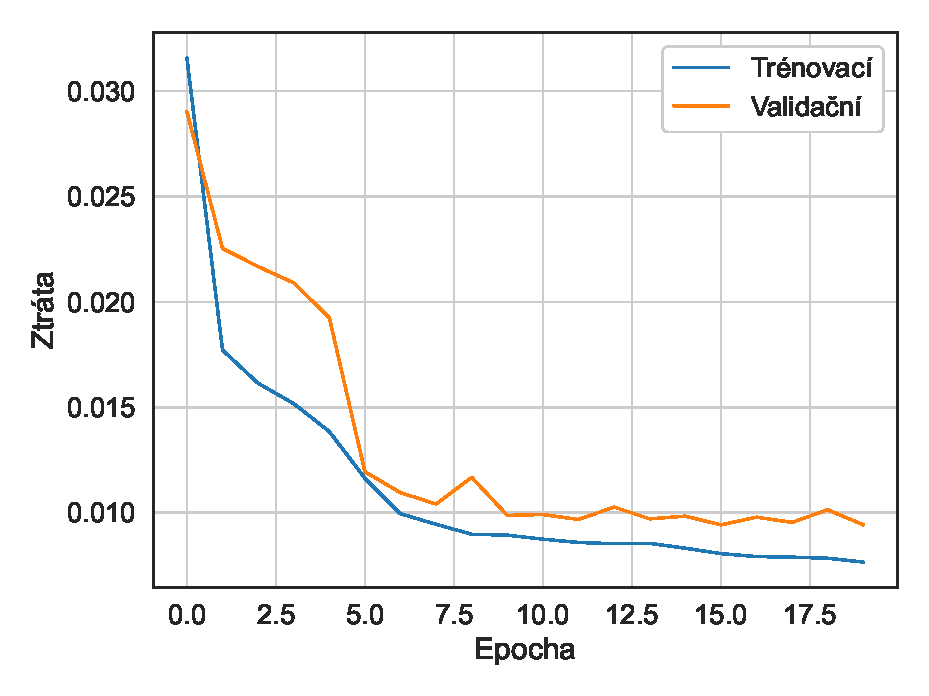
\includegraphics[width=0.6\textwidth]{cnn_lstm_learning_curve.eps}}%
	\caption{Křivka učení finálního CNN-LSTM modelu}
	\label{fig:cnn_lstm_learning_curve}
\end{figure}

Z grafu \ref{fig:cnn_lstm_learning_curve} výše lze vidět, že validační ztráta se ustálila na nízké hodnotě a má tendenci dále klesat k nule. Zároveň je splněna podmínka, že  trénovací a validační ztráty jsou blízko sebe. Tato kombinace naznačuje, že v modelu nedošlo k přeučení a zároveň se model dobře přizpůsobil trénovacím datům.

TODO: Ukázat výřez hodnot

\newpage
\section{Metodika vyhodnocení}\label{section:error-matrix}
Pro kvalitní určení, jak jsou modely úspěšné, je potřeba zavést nějaké metriky. Rozhodnutí bylo ve prospěch tří standardních veličin z matematické statistiky. Jedná se o střední kvadratickou chybu (dále již jen MSE). 

\begin{equation}
	\text{MSE} = \frac{1}{n}\sum_{i=1}^{n}(x_i-y_i)^2 
\end{equation}

a též směrodatná odchylka pro správné jednotky:

\begin{equation}
	\text{RMSE} = \sqrt{\frac{1}{n}\sum_{i=1}^{n}(x_i-y_i)^2}
\end{equation}

Třetí zvolenou veličinou je průměrná absolutní odchylka, která je definována jako:

\begin{equation}
	\text{MAE} = \frac{1}{n}\sum_{i=1}^{n}|x_i-y_i| 
\end{equation}

a pro vyjádření MAE v procentech: 

\begin{equation}
	\text{MAPE} = \frac{1}{n}\sum_{i=1}^{n}|\frac{x_i-y_i}{x_i}| 
\end{equation}

Použití těchto veličin umožňuje poskytnout užitečnou zpětnou vazbu vzhledem k přesnosti predikce a identifikovat případné nedostatky v modelu. Je důležité vyhodnocovat výsledky predikce pomocí více než jedné veličiny, aby se zajistila celková robustnost výsledného modelu.


\chapter{Výsledky}\label{Výsledky}
V této sekci jsou shrnuty a porovnány dosažené výsledky vytrénovaných modelů. Pro porovnání výsledků byla zvolená krátkodobá predikci (max. 30 dnů). Veškeré modely dostavují na vstupu stejné časové úseky. Pro londýnskou datovou sadu to znamená úsek od 28.1. 2014 do 28.2. 2014. A pro datovou sadu zprostředkovanou Albistechem to je úsek od 28. 1. 2023 do 28. 2. 2023.


\begin{table}[!ht]
	\centering
	\caption{Souhrnné výsledky predikce jednoho dne}
	\def\arraystretch{1.2}
	\begin{tabular}{lllllll}
		\hline
		\textbf{Metoda} & \textbf{Rezidence} & \textbf{MSE} & \textbf{RMSE} & \textbf{MAE} & \textbf{MAPE [\%]} \\      \hline
		LSTM            & MAC004431          & TBA               & TBA               & TBA           & TBA              \\ 
		~               & MAC000246          & TBA            & TBA             & TBA            & TBA             \\  
		~               & MAC004387          & TBA            & TBA             & TBA           & TBA            \\ 
		~               & Poštovská 3 - byt 5.02              & TBA            & TBA             & TBA           & TBA \\         
		
		\hline
		
		CNN-LSTM        & MAC004431          & TBA               & TBA               & TBA           & TBA              \\ 
		~               & MAC000246          & TBA            & TBA             & TBA            & TBA             \\  
		~               & MAC004387          & TBA            & TBA             & TBA           & TBA            \\ 
		~               & Poštovská 3 - byt 5.02              & TBA            & TBA             & TBA           & TBA \\         
		
		\hline
		
		
		XGBoost         & MAC004431          & TBA            & TBA             & TBA        &  TBA            \\ 
		~               & MAC000246          & TBA            & TBA             & TBA            & TBA             \\  
		~               & MAC004387          & TBA            & TBA             & TBA           & TBA             \\ 
		~               & Poštovská 3 - byt 5.02              & TBA           & TBA             & TBA           & TBA \\   
		
				\hline
		
		ARIMA           & MAC004431          & TBA            & TBA             & TBA        &  TBA            \\ 
		~               & MAC000246          & TBA            & TBA             & TBA            & TBA             \\  
		~               & MAC004387          & TBA            & TBA             & TBA           & TBA             \\ 
		~               & Poštovská 3 - byt 5.02              & TBA           & TBA             & TBA           & TBA \\   
		

	\end{tabular}
\end{table}



\chapter{Závěr}
Tato práce si kladla za cíl ... 



\printbibliography[title={Použitá literatura}] % sazba seznamu citací 

\addcontentsline{toc}{chapter}{Použitá literatura} % vložení nadpisu do 


\end{document}
